\documentclass[aspectratio=169]{beamer}

\usepackage[utf8]{inputenc}
\usepackage[T1]{fontenc}
\usepackage[turkish,shorthands=off]{babel}
\usepackage{graphicx}
\usepackage{booktabs}
\usepackage{amsmath}
\usepackage{hyperref}
\usepackage{xcolor}

% Hyperref PDF metadata: make line breaks/text formatting safe in PDF strings
\pdfstringdefDisableCommands{%
	\def\\{ }%
	\def\textbf#1{#1}%
}

% --- Title page logos (top-left / top-right) ---
% --- Title page logos (top-left / top-right) ---
\usepackage{tikz}
% Reusable logos row
\newcommand{\IULogos}[1]{%
	\begin{minipage}{\linewidth}
		
\includegraphics[height=#1]{IU-LOGO.png}%
		\hfill%
		
\includegraphics[height=#1]{IUfen-LOGO.png}%
	\end{minipage}%
}

% Title page (top)
\titlegraphic{%
	\vspace*{-1cm}%
	\IULogos{2cm}%
}

% Last slide (bottom) automatically
\addtobeamertemplate{background canvas}{}{%
	\ifnum\insertframenumber=\inserttotalframenumber\relax
		\begin{tikzpicture}[remember picture,overlay]
			\node[anchor=south west,xshift=0.5cm,yshift=0.3cm] at (current page.south west)
				{
\includegraphics[height=2cm]{IU-LOGO.png}};
			\node[anchor=south east,xshift=-0.5cm,yshift=0.3cm] at (current page.south east)
				{
\includegraphics[height=2cm]{IUfen-LOGO.png}};
		\end{tikzpicture}%
	\fi
}

\title{Kalp Anomalilerinin Denetimli Öğrenme ile Sınıflandırılması}
\author{\textbf{İstanbul Üniversitesi, Fen Fakültesi, Bilgisayar Bilimleri Bölümü}\\M. Yusuf Aykut\\İbrahim Abushawish\\Samet Ertuğrul Kurum\\Samet Baturay}
\date{Aralık 2025}
% --- Green main template / accent color ---
\definecolor{MainGreen}{HTML}{2E7D32}

\setbeamercolor{structure}{fg=MainGreen}
\setbeamercolor{frametitle}{bg=MainGreen, fg=white}
\setbeamercolor{title}{fg=MainGreen}

% Optional: blocks
\setbeamercolor{block title}{bg=MainGreen, fg=white}
\setbeamercolor{block body}{bg=MainGreen!5, fg=black}

% Optional: hyperlinks
\hypersetup{colorlinks=true, linkcolor=MainGreen, urlcolor=MainGreen, citecolor=MainGreen}

\begin{document}

\begin{frame}
  \titlepage
\end{frame}

%---------------------------------
\begin{frame}{İçerik}
		\tableofcontents
\end{frame}

%=================================
\section{Giriş}

\begin{frame}{Giriş}
	\begin{itemize}
		\item Elektrokardiyografi (EKG), kalp hastalıklarının erken ve doğru tanısında kritik öneme sahip, kalbin elektriksel aktivitesini kaydeden bir yöntemdir.
		\item EKG sinyalinin morfolojisi ve dalga formlarının süre/genlik özellikleri; miyokard, ritim ve iletim patolojilerinin tespitinde kullanılır.
		\item Yapay zeka ve makine öğrenmesi uygulamalarının klinik pratikte doktorlara yardımcı karar destek sistemleri olarak yaygınlaşması beklenmektedir.
	\end{itemize}
\end{frame}

\begin{frame}{Çalışmanın Amacı}
	\begin{itemize}
		\item PTB-XL+ veri setinden çıkarılmış EKG özniteliklerini kullanarak:
		\begin{itemize}
			\item Normal ve 4 farklı anomali üst sınıfını (NORM, MI, STTC, CD, HYP) sınıflandırmak,
			\item Veri dengesizliği sorununa yönelik yöntemleri incelemek ve karşılaştırmak,
		\end{itemize}
		\item Denetimli öğrenme temelli, açıklanabilir bir sınıflandırma hattı tasarlamak ve değerlendirmek.
	\end{itemize}
\end{frame}

%=================================
\section{Literatür Taraması}

\begin{frame}{Literatürden Örnek Çalışma 1}
		PTB-XL ve Georgia ECG veri setlerinde, sol ventriküler hipertrofi (LVH) tespiti \cite{taconne2024-lvh}:
	\begin{itemize}
		\item Yalnızca NORMAL ve LVH etiketli kayıtlar kullanılmış, düşük kaliteli sinyaller elenmiştir.
		\item Özellik çıkarımı araştırmacılar tarafından yapılmış; Logistic Regresyon, Rastgele Orman (RF) ve Destek Vektör Makinesi (SVM) denenmiştir.
		\item RF ve SVM ile \%87 üzerinde duyarlılık ve özgüllük elde edilmiştir.
		\item Veri dengesizliği: normal sınıfta downsampling, 100 kez tekrarlı eğitim ve ensemble ile telafi edilmiştir.
		\item SFFS ile en önemli 5 özellik seçilmiş, basitleştirilmiş modeller kurulmuştur.
	\end{itemize}
\end{frame}

\begin{frame}{Literatürden Örnek Çalışma 2}
		Miyokardiyal Enfarktüs tespiti için klasik ML ve CNN karşılaştırması \cite{osterlund2025-mi-ptbxl}:
	\begin{itemize}
		\item 7 klasik model: KNN, SVM, RF, XGBoost, Decision Tree, Gaussian Naive Bayes vb.
		\item Eksik verilerde \texttt{SimpleImputer}, ağaç dışı modellerde \texttt{StandardScaler} kullanılmıştır.
		\item PTB-XL'den yalnızca NORM ve MI etiketli, 100 Hz, 12 derivasyonlu EKG'ler alınmıştır.
		\item Veri MI referanslı 70/15/15 (train/val/test) bölünmüş, yalnızca eğitim seti dengelenmiştir.
		\item En yüksek doğruluk: XGBoost ile \%89; ardından SVM ve RF \%88 düzeyinde.
	\end{itemize}
\end{frame}

\begin{frame}{Literatürden Örnek Çalışma 3}
		PhysioNet/CinC 2020 Challenge, 12 derivasyonlu EKG ve XGBoost \cite{raipal2020-xgboost-cinc}:
	\begin{itemize}
		\item Çoklu etiket problemi için her etiket için ayrı bir ikili XGBoost modeli eğitilmiştir.
		\item Sınıf dengesizliği: undersampling + K-fold çapraz doğrulama ile ele alınmıştır.
		\item Çıktı olasılıkları için sınıf bazlı, yüksek eşik değerleri (ör. 0.9) kullanılmıştır.
		\item Challenge skoru 0.155 olup, katılan takımlar arasında orta sıralarda yer almıştır.
	\end{itemize}
\end{frame}

%=================================
\section{Yöntem}

\subsection{Veri Seti Tanımı}

\begin{frame}{PTB-XL+ Veri Seti}
	\begin{itemize}
		\item PTB-XL+: 12 derivasyonlu EKG dalga formlarından üç analiz aracının (GE Marquette 12SL, Uni-G, ECGDeli) çıkardığı öznitelikleri içerir.
		\item Süreler, genlikler, segment başlangıç/bitişleri, alanlar ve vektörkardiyografik ölçümler gibi klinik olarak yorumlanabilir özellikler sunar.
		\item 12SL'nin otomatik tanı ifadeleri ve PTB-XL etiketlerinin SNOMED CT eşlemeleri mevcuttur.
		\item Bu sayede, modeller klinisyen etiketleri ile otomatik ifadeler arasında karşılaştırmalı olarak eğitilip değerlendirilebilir \cite{wagner2023-ptbxlplus}.
	\end{itemize}
\end{frame}

\begin{frame}{PTB-XL Demografik ve Tanısal Özellikler}
	\begin{itemize}
		\item 18.869 hastadan, 10 saniyelik 21.799 klinik 12 derivasyonlu EKG kaydı (500 ve 100 Hz sürümleri mevcut).
		\item Yaş dağılımı 40--80 yaşta yoğun, ortalama 62.8 yıl; ortalama boy 166.7 cm, kilo 71.0 kg.
		\item Cinsiyet: \%52.1 erkek, \%47.9 kadın.
		\item Veri çerçevesi: 21.388 kayıt, 793 sütun (750 sayısal, 42 tamsayı, 1 kategorik).
	\end{itemize}
\end{frame}

\begin{frame}{Sınıf Dağılımları ve Dengesizlik}
	\begin{itemize}
		\item Beş üst sınıf: Normal, MI, ST/T Değişikliği (STTC), İletim Bozukluğu (CD), Hipertrofi (HYP).
		\item Örnek dağılımı yaklaşık olarak:
		\begin{itemize}
			\item NORM: \%44.5
			\item MI: \%25.4
			\item STTC: \%13.2
			\item CD: \%10.9
			\item HYP: \%6.1
		\end{itemize}
		\item Belirgin sınıf dengesizliği mevcuttur: normal kayıtlar veri setinin neredeyse yarısını oluştururken, HYP oldukça azdır.
		\item Bu durum, modellerin azınlık sınıfları öğrenmesini zorlaştırabilir ve metriklerin yanıltıcı şişmesine yol açabilir.
	\end{itemize}
\end{frame}

\subsection{Ön İşleme}

\begin{frame}{Ön İşleme: Genel Hatlar}
	\begin{itemize}
		\item Klinik üst bilgi tablosu ile 12-lead öznitelik tablosu \texttt{ecg\_id} üzerinden birleştirilmiştir.
		\item SCP-ECG tanı kodları 5 ana üst sınıfa (NORM, MI, STTC, CD, HYP) dönüştürülmüştür.
		\item Herhangi bir tanı sınıfına girmeyen veya etiketi olmayan 411 kayıt çıkarılmış, 21.388 kayıt kalmıştır.
		\item Veri sızıntısını önlemek için tüm dönüşümler eğitim/val/test ayrımından \emph{sonra} ve eğitim seti üzerinde fit edilmiştir \cite{kuhn2013-applied-predictive-modeling}.
	\end{itemize}
\end{frame}

\begin{frame}{Eksik Veriler: Demografi ve EKG}
	\begin{itemize}
		\item Demografik değişkenler:
			\begin{itemize}
				\item Boy: \%67.65 eksik, kilo: \%56.21 eksik; bu nedenle modelden tamamen çıkarılmıştır.
			\end{itemize}
		\item EKG öznitelikleri:
			\begin{itemize}
				\item \texttt{T\_AxisFront\_Global} ve \texttt{R\_AxisFrontal\_Global}: çok az sayıda eksik; ilgili kayıtlar silinmiştir.
				\item P dalgası ile ilişkili \texttt{P\_On\_Global}, \texttt{P\_Off\_Global}, \texttt{P\_Dur\_Global}, \texttt{P\_AxisFront\_Global}, \texttt{PR\_Int\_Global}, \texttt{HR\_Atrial\_Global}: yaklaşık \%8 eksik.
			\end{itemize}
		\item Satır bazlı eksiklik oranı \%1'in altında olduğundan, satır silme yalnızca etiketi eksik örneklerle sınırlı tutulmuştur.
	\end{itemize}
\end{frame}

\begin{frame}{Figür 1: Eksik Değer Analizi}
	\centering
	\resizebox{0.95\linewidth}{!}{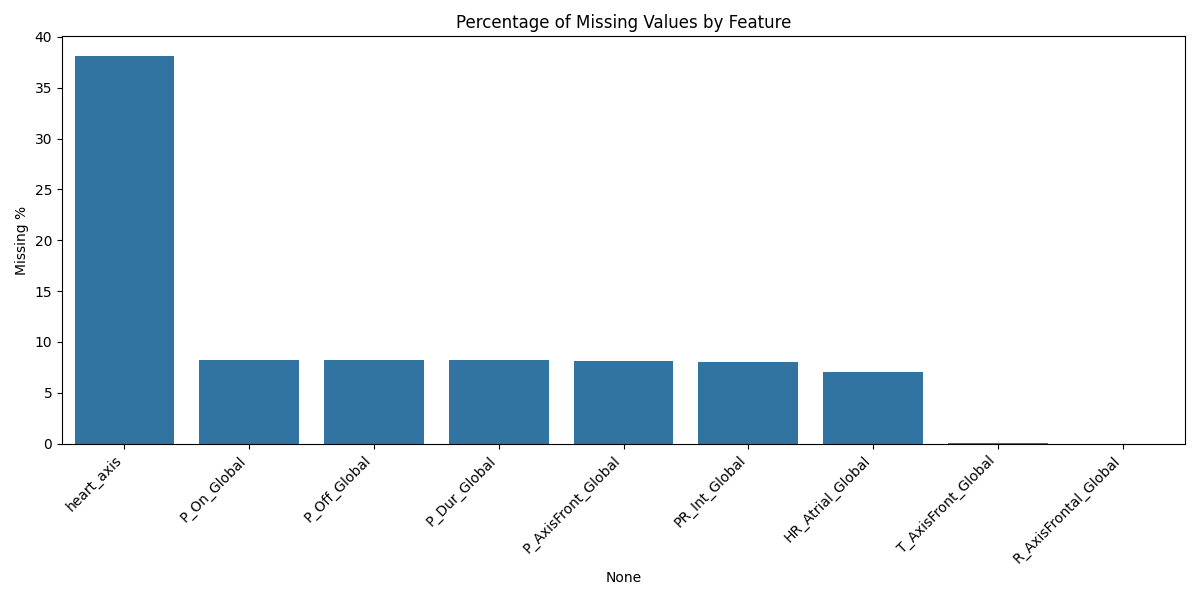
\includegraphics{../reports/missing_data_analysis/missing_values_barplot.png}}
\end{frame}

\begin{frame}{Figür 2: Eksik Değer Analizi}
	\centering
	\resizebox{0.95\linewidth}{!}{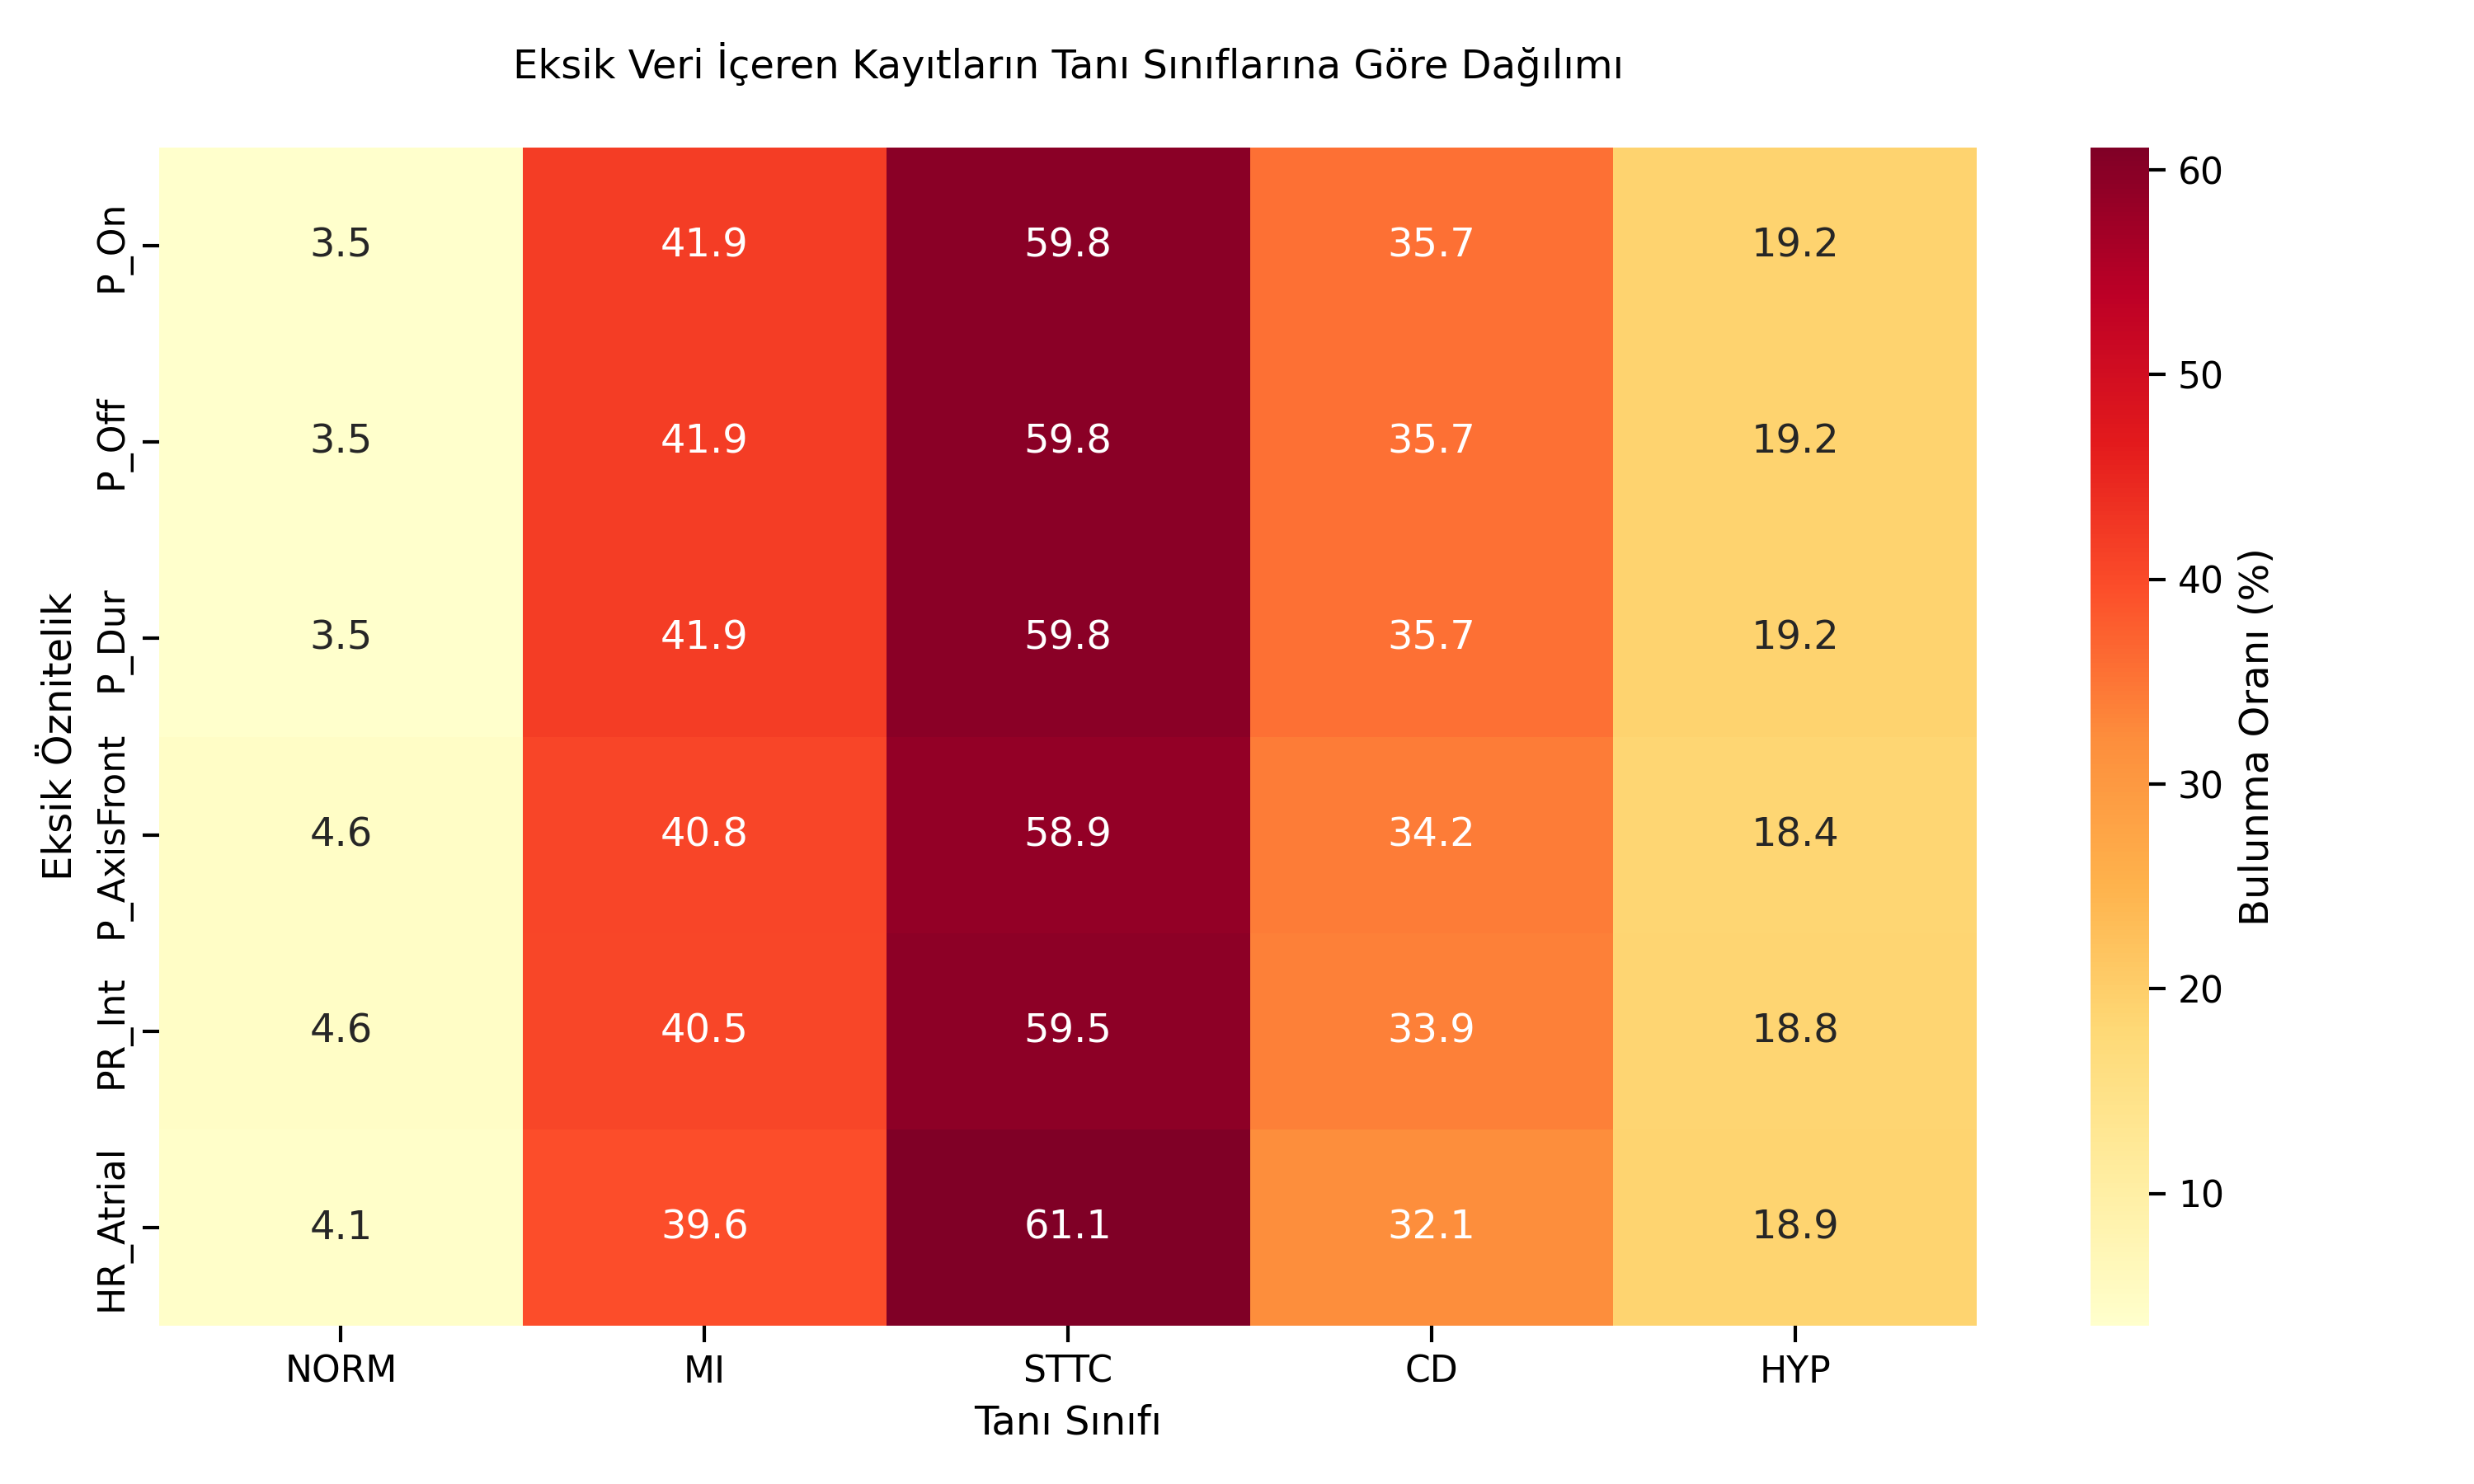
\includegraphics{../reports/missing_data_analysis/missingness_diagnosis_heatmap_paper.png}}
\end{frame}

\begin{frame}{Eksik Veri Stratejisi}
	\begin{itemize}
		\item P dalgası ile ilişkili özniteliklerdeki eksiklik, MI ve STTC sınıflarında anlamlı biçimde daha sık görülmektedir \cite{rubin1976-missing-data}.
		\item Bu nedenle eksiklik, yalnızca teknik bir sorun değil, fizyolojik bir işaret (ör. atriyal fibrilasyon) olarak ele alınmıştır.
		\item Strateji:
		\begin{itemize}
			\item P dalgası öznitelikleri için: sabit değer (0.0) + \texttt{is\_missing} bayrağı ile kodlama.
			\item Diğer sayısal öznitelikler için: eğitim seti medyanı + \texttt{is\_missing} bayrağı.
			\item \texttt{heart\_axis}: \%38 eksiklik ve düşük ek bilgi nedeniyle tamamen çıkarılmıştır.
		\end{itemize}
	\end{itemize}
\end{frame}

\begin{frame}{Veri Bölme, İmputasyon ve Ölçekleme}
	\begin{itemize}
		\item Veri, \texttt{strat\_fold} etiketine göre üç kümeye ayrılmıştır:
		\begin{itemize}
			\item Eğitim: 17.084 örnek (\%79.9)
			\item Doğrulama: 2.146 örnek (\%10.0)
			\item Test: 2.158 örnek (\%10.1)
		\end{itemize}
		\item Eksik değer doldurma (imputasyon):
		\begin{itemize}
			\item Sadece eğitim seti üzerinde \texttt{SimpleImputer(strategy="median")} fit edilmiştir.
			\item Aynı imputer, doğrulama ve test kümelerine uygulanmıştır.
		\end{itemize}
		\item Ölçekleme:
		\begin{itemize}
			\item Sayısal sütunlar için \texttt{StandardScaler} yalnızca eğitim setinde fit edilmiştir.
			\item Eksiklik bayrakları ölçekleme dışında tutulmuştur.
		\end{itemize}
	\end{itemize}
\end{frame}

\begin{frame}{Figür 3: Splitlere Göre Sınıf Dağılımı}
	\centering
	\resizebox{0.86\linewidth}{!}{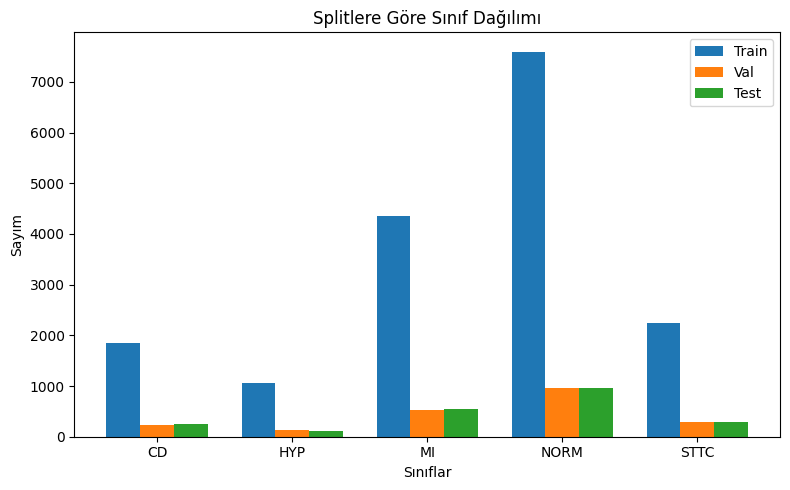
\includegraphics{../reports/data_summary/class_distribution_splits.png}}
\end{frame}



\begin{frame}{Sınıf Dengesizliği}
	\begin{itemize}
		\item Eğitim/val/test kümeleri oluşturulduktan sonra sınıf dağılımları incelenmiş, dengesizliğin korunduğu görülmüştür.
		\item Dengesizliğin model üzerindeki etkisini azaltmak için iki ana yaklaşım kullanılmıştır:
		\begin{itemize}
			\item Sınıf ağırlıkları (\texttt{class\_weight="balanced"})
			\item Rastgele undersampling (yalnızca eğitim kümesinde)
		\end{itemize}
		\item Sınıf ağırlıkları, yalnızca eğitim verisi üzerinden hesaplanmış ve azınlık sınıfların kayıp fonksiyonuna katkısı artırılmıştır.
	\end{itemize}
\end{frame}

\begin{frame}{Sınıf Dengesizliği (Devam)}
	\begin{itemize}
		\item oversampling yöntemleri (SMOTE, ADASYN vb.) denenmiş ancak başarılı sonuçlar elde edilmemiştir.
		\begin{itemize}
			\item Çoklu sınıf yapısı ve yüksek boyutlu öznitelik uzayı nedeniyle sentetik örnekler gerçekçi değildir.
			\item veri sayısını değiştirmedeğitilen modeller oversampling ile aynı aynı sayılabilecek performans göstermiştir.
		\end{itemize}
	\end{itemize}
\end{frame}

\subsection{Öznitelik Seçimi}

\begin{frame}{Öznitelik Seçimi: Varyans Eşikleme}
	\begin{itemize}
		\item İlk adım: \emph{Variance Threshold} yöntemi ile varyansı çok düşük, sabite yakın öznitelikler elenmiştir.
		\item Varyansları 0.05'in altında olan öznitelikler çıkarılmış; 793 özelliğin 186 tanesi bu nedenle elenmiştir.
		\item Böylece bilgi katkısı sınırlı, durağan ve gürültülü özellikler modelleme dışına alınmıştır.
	\end{itemize}
\end{frame}

%C:\Users\Pc\Desktop\LOCALS\ML_PTB-XL\PTB-XL-Heart-Anomaly-Diagnosis-Project\reports\feature_selection\variance_histogram.png
\begin{frame}{Figür 3: Varyans Dağılımı}
	\centering
	\resizebox{0.95\linewidth}{!}{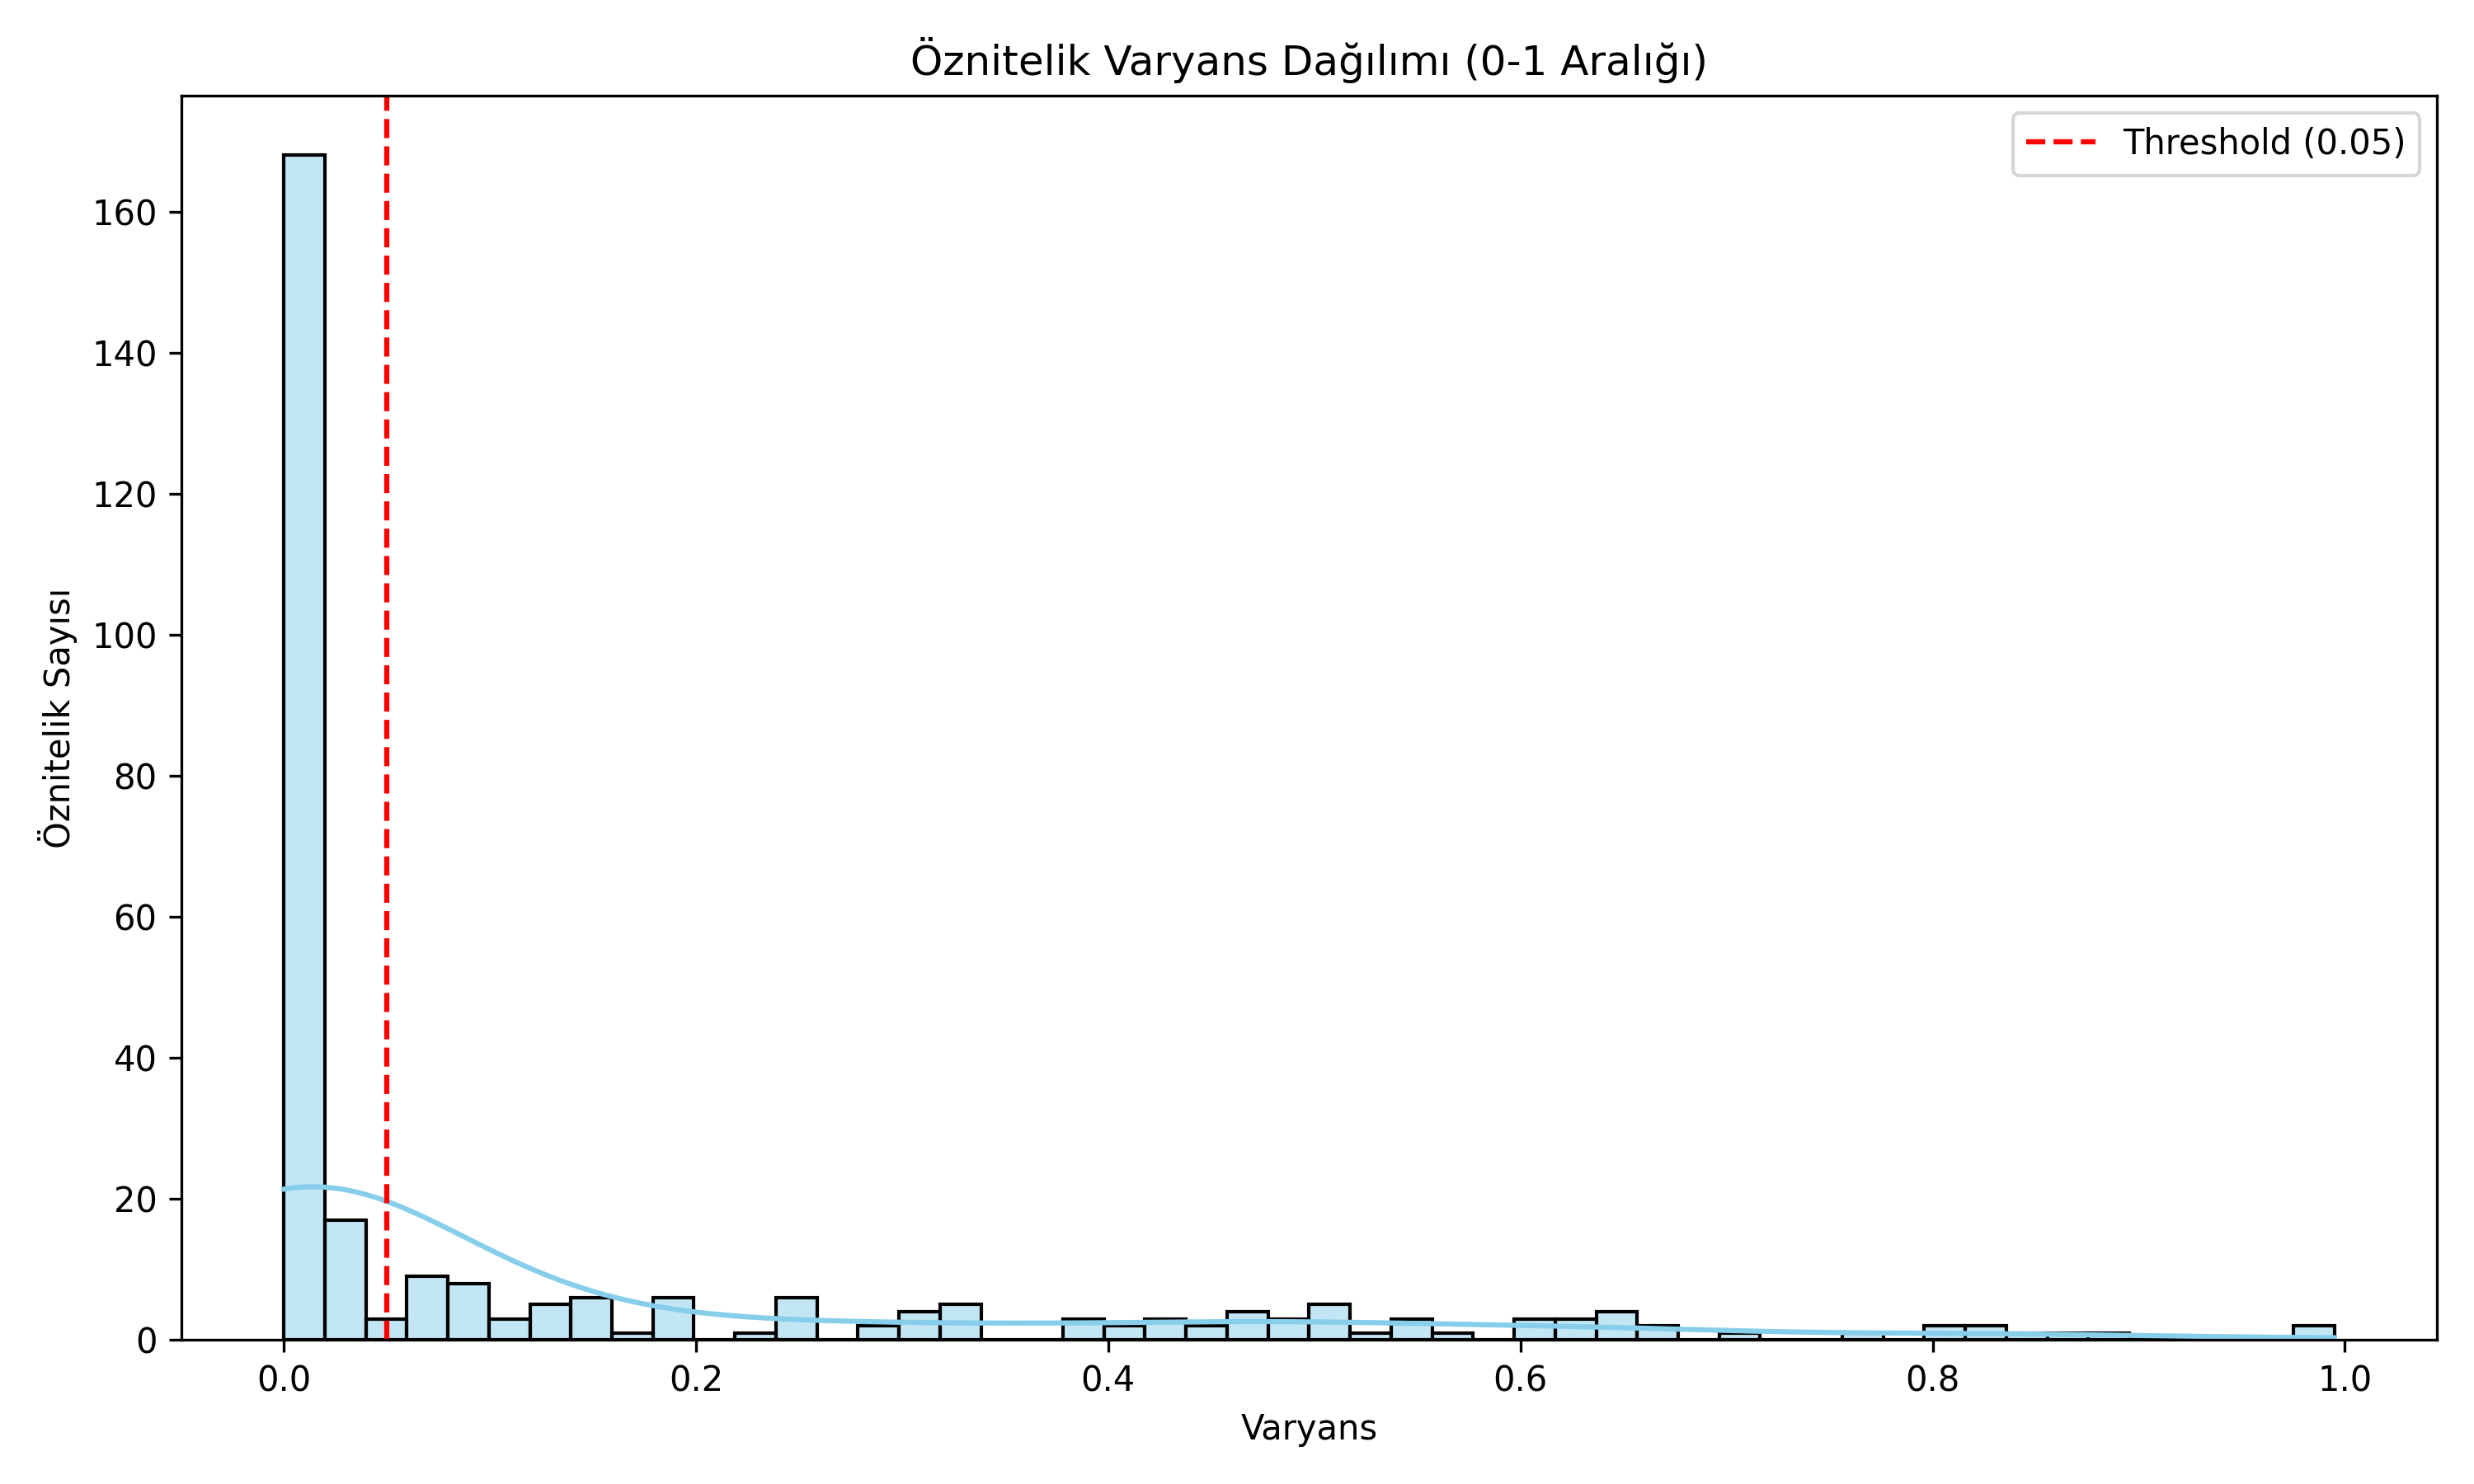
\includegraphics{../reports/feature_selection/variance_histogram.png}}
\end{frame}


\begin{frame}{Öznitelik Seçimi: Random Forest Önem Skorları}
	\begin{itemize}
		\item İkinci adım: \texttt{RandomForestClassifier} ile öznitelik önem sıralaması yapılmıştır.
		\item Model ayarları: \texttt{n\_estimators=250}, \texttt{max\_depth=12}, \texttt{random\_state=42}, \texttt{n\_jobs=-1}.
		\item Her ağaçta kullanılan bölünmelerdeki bilgi kazançları toplanarak normalize edilmiş önem skorları elde edilmiştir \cite{breiman2001-rf}.
		\item En yüksek skoru alan 50, 100 ve 200 öznitelik; üç ayrı alt küme (Top-50, Top-100, Top-200) olarak tanımlanmıştır.
		\item Bu alt kümelerle ayrı RF modelleri eğitilerek özellik sayısının performansa ve overfitting'e etkisi incelenmiştir.
	\end{itemize}
\end{frame}

\begin{frame}{Figür 4: Öznitelik Seçimi ve Önem Düzeyleri}
	\centering
	\begin{columns}
		\begin{column}{0.48\textwidth}
			\begin{figure}
				\centering
				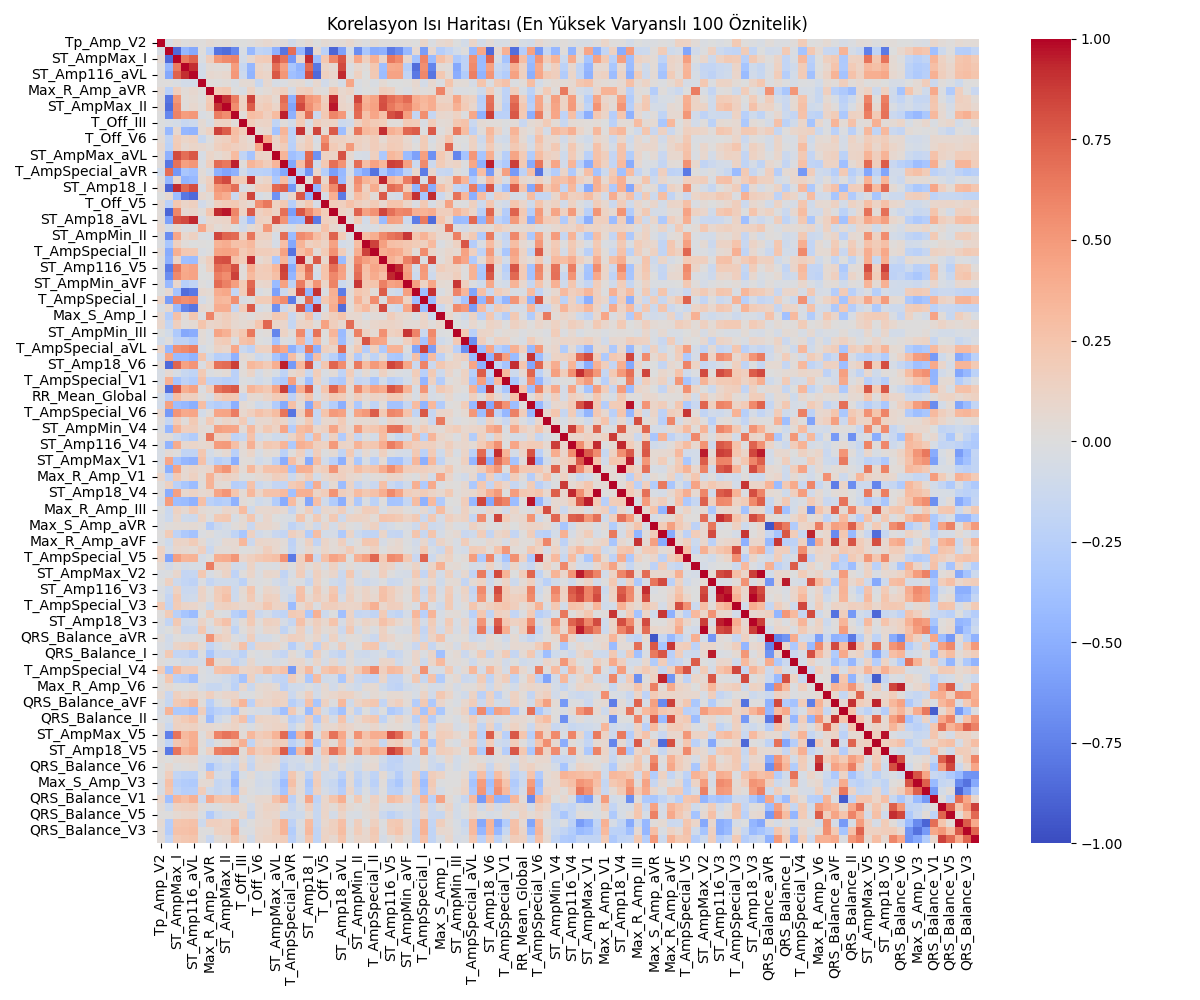
\includegraphics[width=\linewidth]{../reports/feature_selection/correlation_heatmap_top100_variance.png}
				\caption{Top-100 Öznitelik Korelasyon Isı Haritası filtreleme öncesi (varyanslı)}
			\end{figure}
		\end{column}
		\begin{column}{0.48\textwidth}
			\begin{figure}
				\centering
				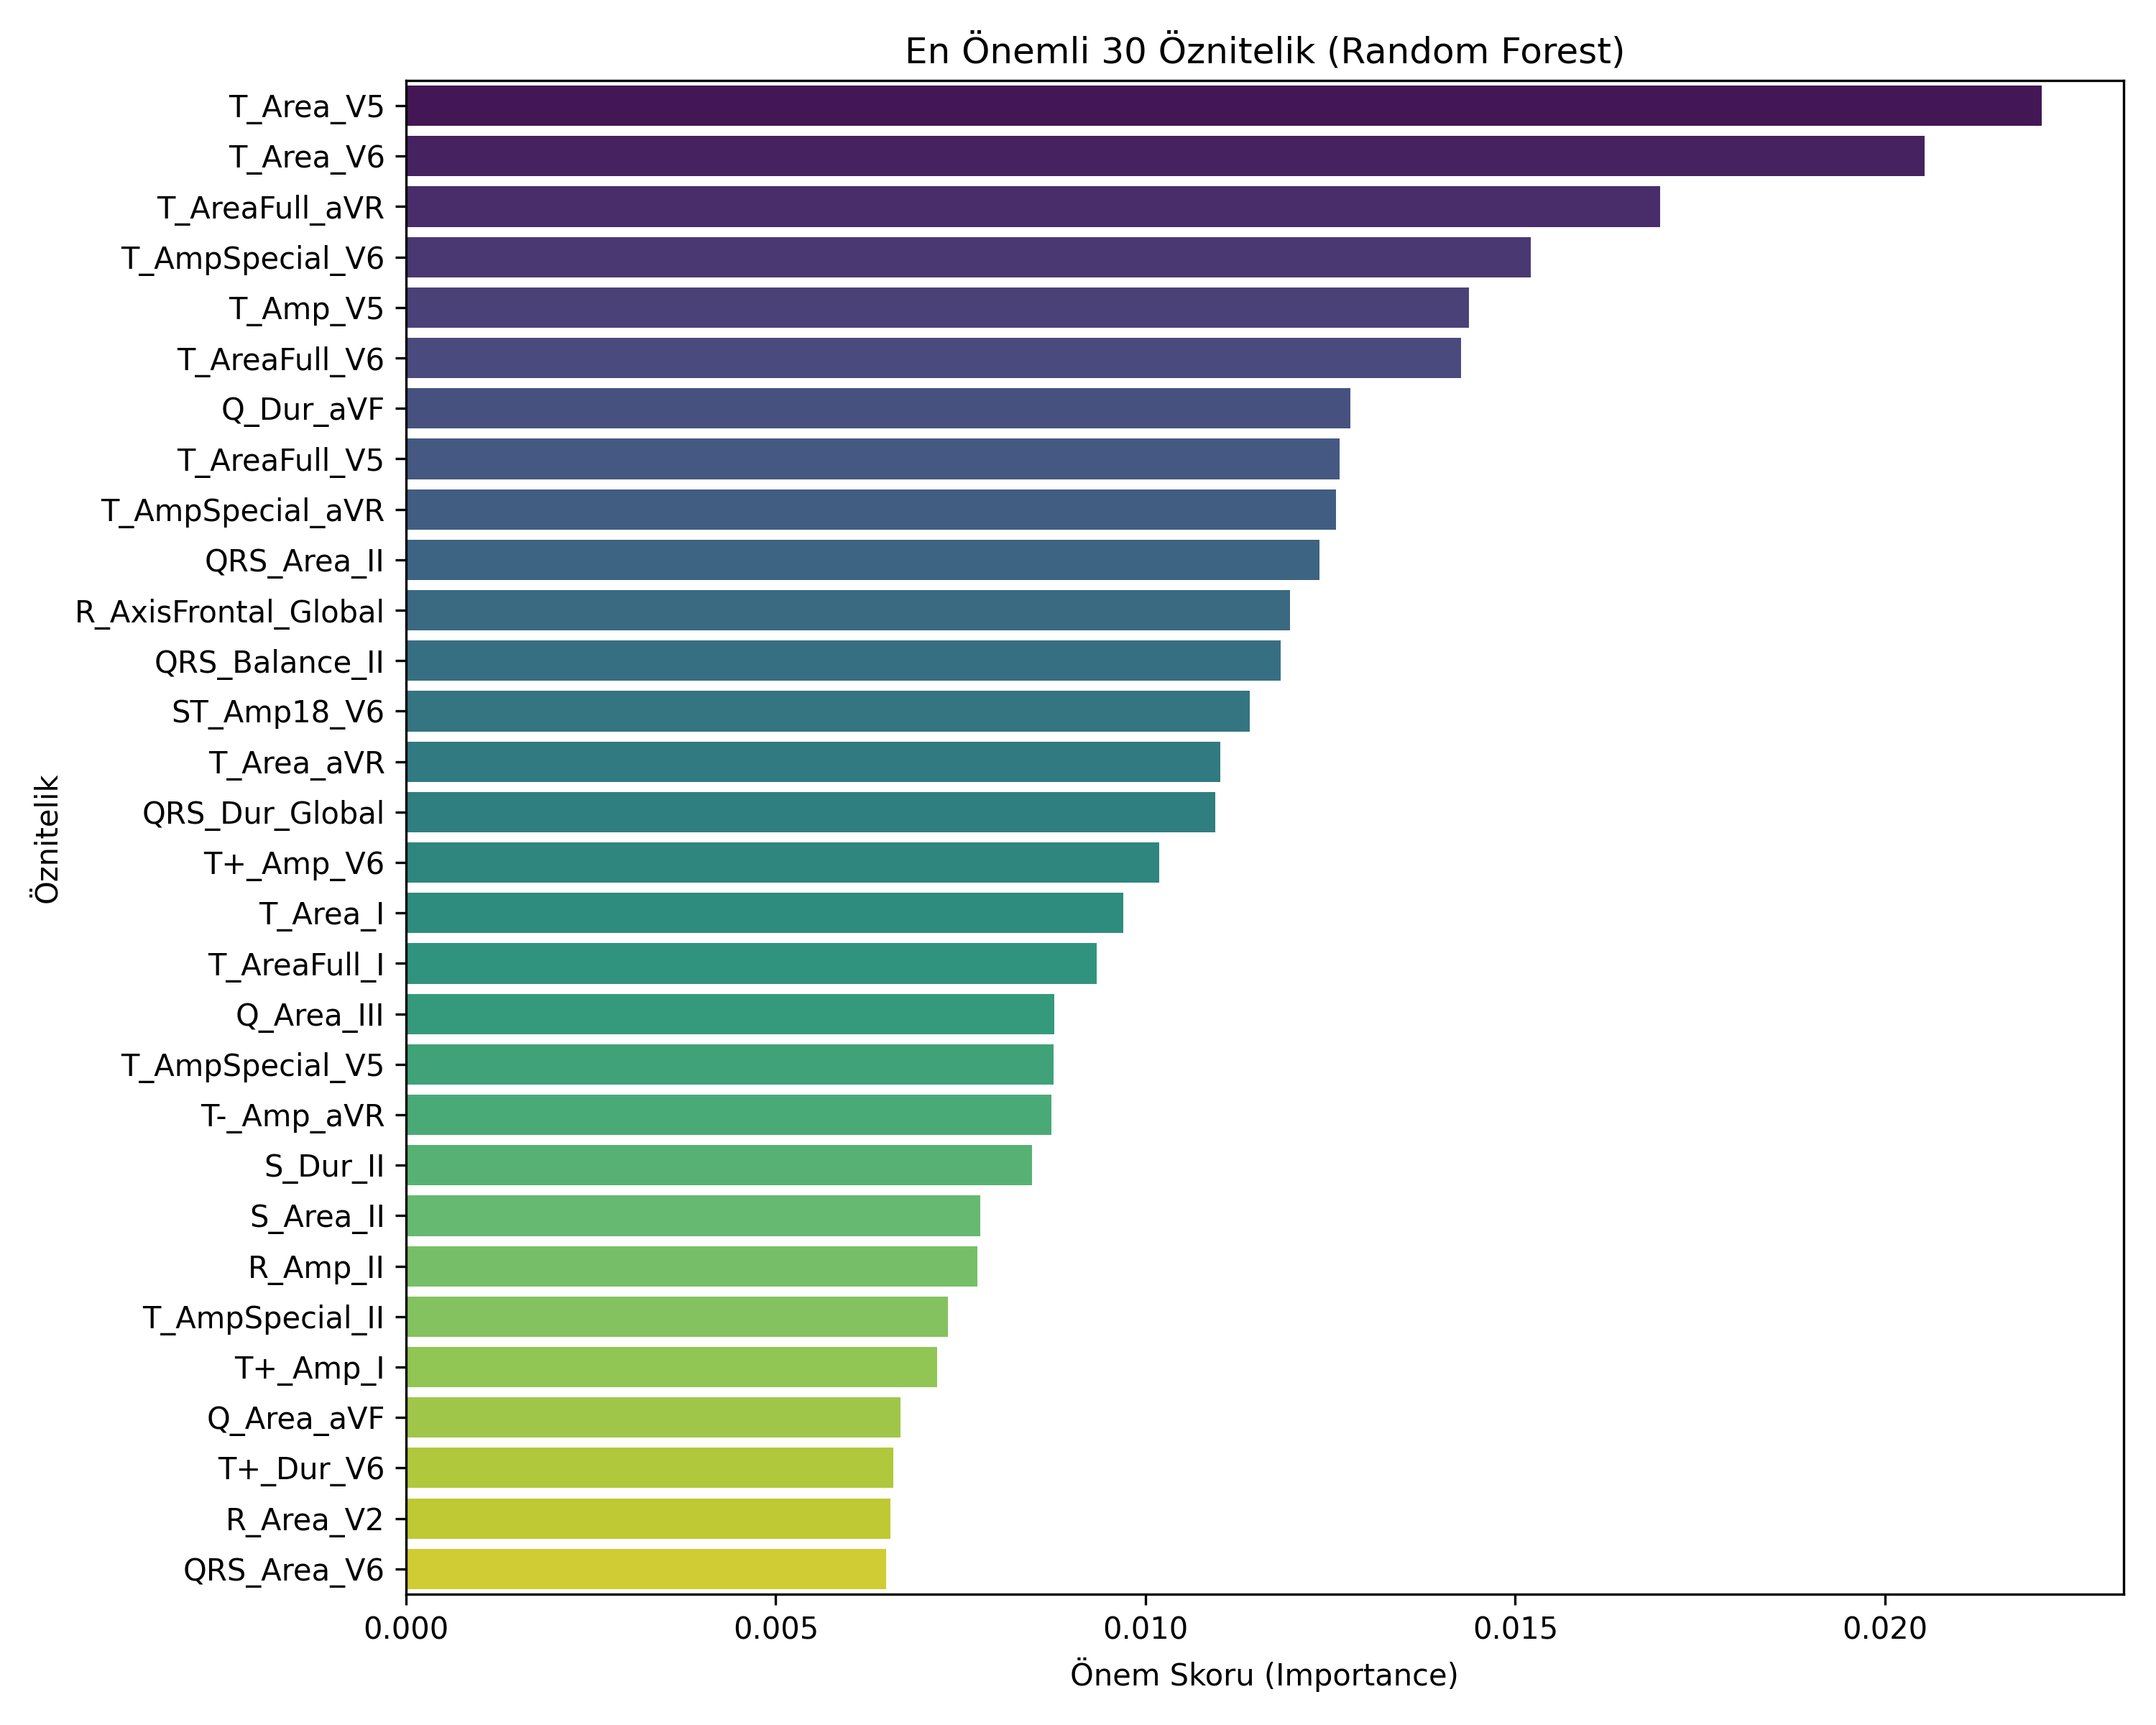
\includegraphics[width=\linewidth]{../reports/feature_selection/rf_importance_top30_final.png}
				\caption{RF Model Bazlı Önem Düzeyleri}
			\end{figure}
		\end{column}
	\end{columns}
	\vspace{0.5cm}
	\footnotesize{Not: En yüksek skora sahip öznitelikler (Top-50, Top-100, Top-200) seçilerek model eğitiminde kullanılmıştır.}
\end{frame}

\begin{frame}{Figür 5: Korelasyon Isı Haritası (Top-100) filtreleme sonrası}
	\centering
	\begin{figure}
		\centering
		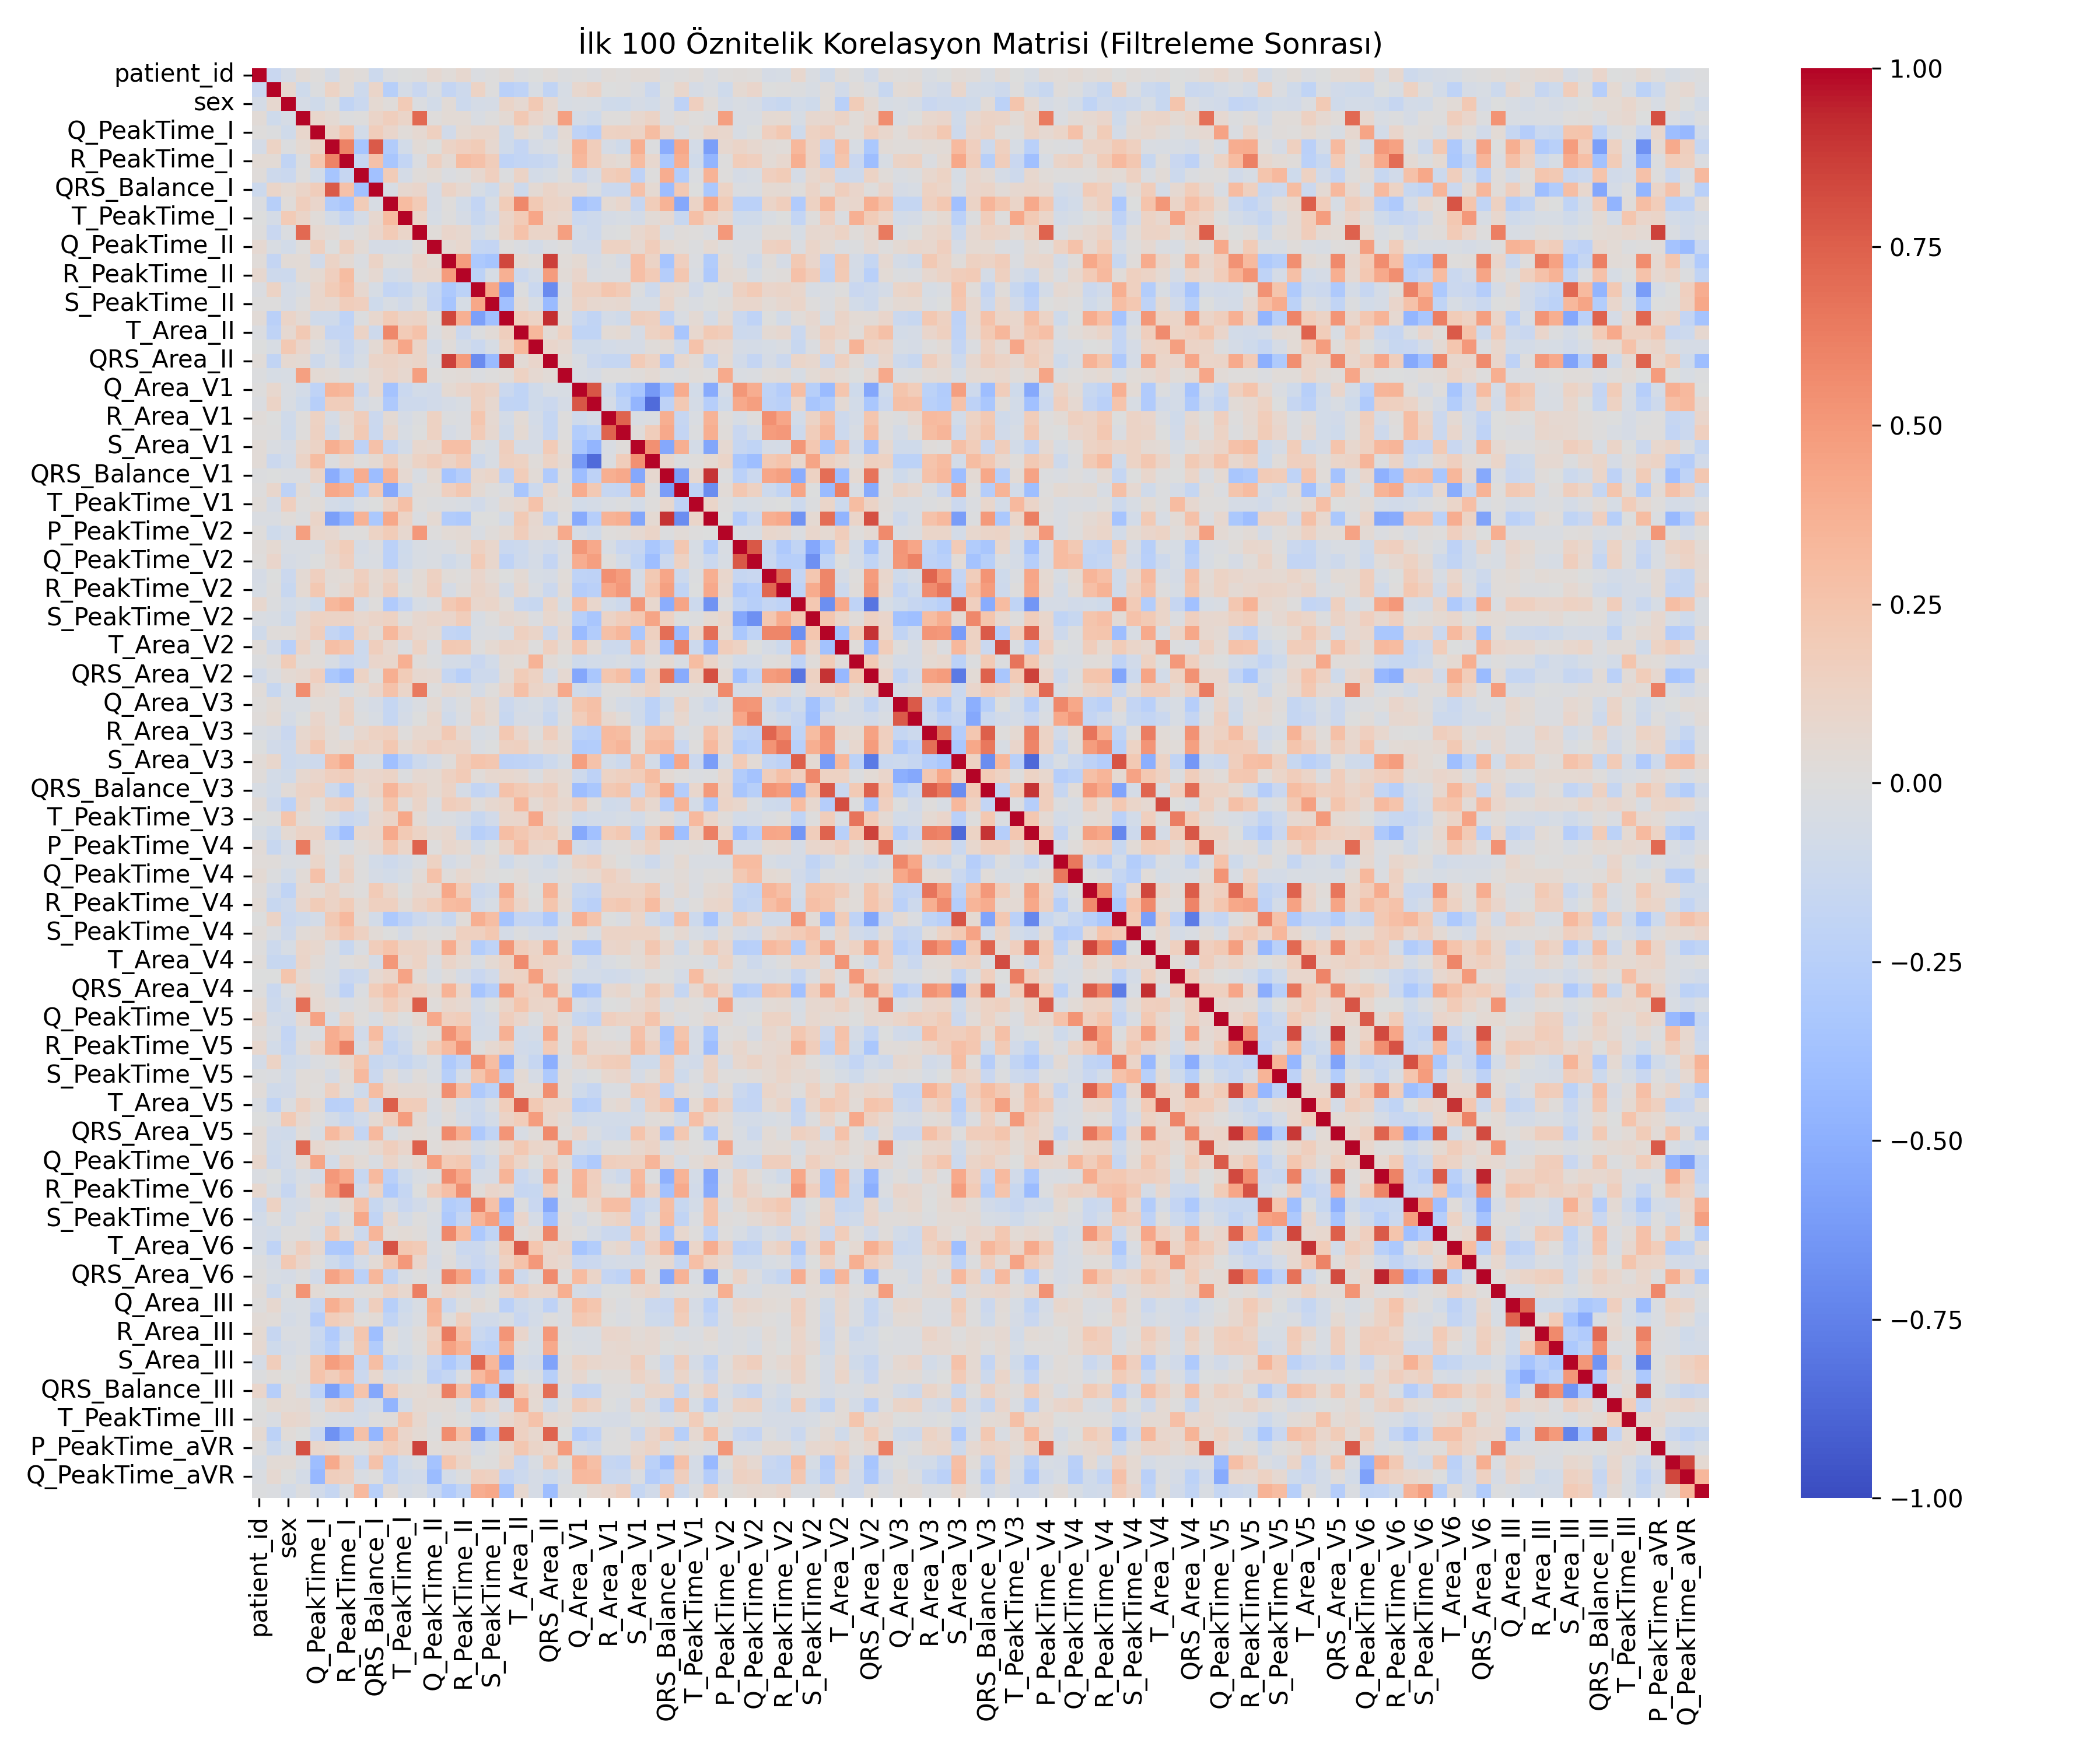
\includegraphics[height=0.75\textheight]{../reports/feature_selection/correlation_heatmap_sample.png}
		\caption{Top-100 Öznitelik Korelasyon Isı Haritası filtreleme sonrası}
	\end{figure}
\end{frame}

\subsection{Model Seçimi ve Eğitim}

\begin{frame}{Model Seçimi: Random Forest}
	\begin{itemize}
		\item Bu çalışmada sınıflandırıcı olarak yalnızca Random Forest (RF) kullanılmıştır \cite{breiman2001-rf}.
		\item Tercih nedenleri:
		\begin{itemize}
			\item Nonlineer ilişkileri yakalayabilmesi,
			\item Yüksek boyutlu öznitelik uzaylarında güçlü performans,
			\item Ölçeklemeye görece duyarsız oluşu,
			\item Öznitelik önem skorları ile yorumlanabilirlik sunması.
		\end{itemize}
		\item Temel hiperparametreler tüm deneylerde sabitlenmiştir:
		\begin{itemize}
			\item \texttt{n\_estimators=250}, \texttt{max\_depth=12}, \texttt{random\_state=42}, \texttt{n\_jobs=-1}.
		\end{itemize}
	\end{itemize}
\end{frame}
\begin{frame}{Random Forest: Çalışma Prensibi ve Mantığı}
	\begin{itemize}
		\item \textbf{Temel fikir:} Tek bir karar ağacı yerine, \emph{çok sayıda} farklı karar ağacını bir araya getirerek (ensemble) daha kararlı ve genellenebilir bir model elde etmek.
		
		\item \textbf{Bagging (Bootstrap Aggregation):}
		Her ağaç, eğitim verisinden \emph{tekrar seçmeli} (bootstrap) örnekleme ile oluşturulan farklı bir alt veri kümesiyle eğitilir.
		\begin{itemize}
			\item Böylece ağaçlar aynı veriyi görse bile farklı örüntüler öğrenir.
			\item Amaç, tek ağaçların \textbf{yüksek varyansını} azaltmaktır.
		\end{itemize}
		
		\item \textbf{Rastgele öznitelik altkümesi:}
		Her düğümde bölme yapılırken tüm öznitelikler yerine rastgele seçilmiş bir alt küme değerlendirilir.
		\begin{itemize}
			\item Ağaçlar arası korelasyonu düşürür, çeşitliliği artırır.
			\item Benzer güçlü özniteliklerin tüm ağaçları domine etmesini engeller.
		\end{itemize}
		
		\item \textbf{Birleştirme (Aggregation):} Sınıflandırmada ağaç çıktıları çoğunluk oyu / olasılık ortalaması ile birleştirilir \cite{breiman2001-rf}:
		\[
		\hat{p}(y=c\mid x)=\frac{1}{T}\sum_{t=1}^{T} p_t(y=c\mid x), \qquad
		\hat{y}=\arg\max_c \hat{p}(y=c\mid x)
		\]
		
		\item \textbf{Yan ürünler:} \emph{Out-of-bag} (OOB) örnekleriyle hızlı hata tahmini ve öznitelik önem skorları (feature importance) elde edilebilir.
	\end{itemize}
\end{frame}
\begin{frame}{Dengesizlik Deney Tasarımı}
	\begin{itemize}
		\item Aynı RF modeli altında iki değişkenin etkisi incelenmiştir:
		\begin{itemize}
			\item Öznitelik sayısı: Top-50 / Top-100 / Top-200
			\item Dengesizlik stratejisi: sınıf ağırlıkları vs. undersampling
		\end{itemize}
		\item Senaryolar:
		\begin{itemize}
			\item \textbf{CW-50 / CW-100 / CW-200}: \texttt{class\_weight="balanced"} yaklaşımı \cite{he2009-imbalanced-data} ile üç farklı öznitelik seti.
			\item \textbf{US-200}: Sadece eğitim setinde rastgele undersampling \cite{liu2008-exploratory-undersampling} + Top-200 öznitelik.
		\end{itemize}
		\item Olasılıksal çıktılar için sınıf bazlı eşikler, F1 skorunu maksimize edecek şekilde 0.01 aralıklarla taranmıştır.
	\end{itemize}
\end{frame}

\begin{frame}{Kodlama Ortamı}
	\begin{itemize}
		\item Tüm analiz ve deneyler Python 3 ortamında, açık kaynak kütüphaneler kullanılarak gerçekleştirilmiştir.
		\item Bağımlılıklar \texttt{requirements.txt} ile yönetilmiştir: \texttt{pandas}, \texttt{numpy}, \texttt{scikit-learn}, \texttt{matplotlib}, \texttt{seaborn}.
		\item Deney akışı modülerleştirilmiştir: ön işleme hattı (\texttt{preprocessing/pipeline.py}), model eğitimi ve metrik/çizimler (\texttt{training/train\_models.py}), makale figürleri (\texttt{figures/generate\_figures.py}).
		\item Kod ve deney çıktıları sürüm kontrolü ile yönetilmiş ve herkese açık repo olarak paylaşılmıştır: \href{https://github.com/AykutN/PTB-XL-Heart-Anomaly-Diagnosis-Project}{github.com/AykutN/PTB-XL-Heart-Anomaly-Diagnosis-Project}
	\end{itemize}
\end{frame}

%=================================
\section{Sonuçlar}

\begin{frame}{Genel Performans (Eğitim / Val)}
	\begin{itemize}
		\item RF + Top-50: Accuracy \%55.33, Precision \%67.64, Recall \%76.53, F1 \%71.53, ROC-AUC 0.904.
		\item RF + Top-100: Accuracy \%58.43, Precision \%71.29, Recall \%73.68, F1 \%72.39, ROC-AUC 0.909.
		\item RF + Top-200: Accuracy \%58.85, Precision \%71.30, Recall \%75.60, F1 \%73.21, ROC-AUC 0.915.
		\item RF + Top-200 + Ensemble: Recall artarken (yaklaşık \%78.6), doğruluk ve precision bir miktar düşmüş; F1 kazancı sınırlı kalmıştır.
	\end{itemize}
\end{frame}

\begin{frame}{Öznitelik Sayısının Etkisi}
	\begin{itemize}
		\item Top-50'den Top-200'e geçiş, Accuracy ve F1 metriklerinde artış sağlamıştır.
		\item ROC-AUC tüm senaryolarda 0.90 üzerinde, Top-200 ile 0.915 seviyesine ulaşmaktadır.
		\item Bu sonuç, PTB-XL+'ın sayısal EKG özniteliklerinin sınıfları ayırma gücünün yüksek olduğunu göstermektedir.
	\end{itemize}
\end{frame}

\begin{frame}{Sınıf Bazlı Sonuçlar (CW-200)}
	\begin{itemize}
		\item NORM: Eşik 0.30; Precision \%79.27, Recall \%92.11, F1 \%85.21.
		\item MI: Eşik 0.45; Precision \%74.91, Recall \%72.73, F1 \%73.80.
		\item STTC: Eşik 0.46; Precision \%69.24, Recall \%79.08, F1 \%73.84.
		\item CD: Eşik 0.45; Precision \%76.87, Recall \%70.36, F1 \%73.47.
		\item HYP: Eşik 0.43; Precision \%56.23, Recall \%63.74, F1 daha düşük seviyededir.
	\end{itemize}
\end{frame}

\begin{frame}{ROC-AUC Değerleri}
	\begin{itemize}
		\item ROC eğrileri tüm sınıflar için yüksek ayrıştırma gücü göstermektedir:
		\begin{itemize}
			\item NORM: AUC 0.938
			\item MI: AUC 0.923
			\item STTC: AUC 0.929
			\item CD: AUC 0.901
			\item HYP: AUC 0.883
		\end{itemize}
		\item HYP diğer sınıflara göre daha zor bir sınıftır; buna rağmen AUC'nin 0.88 üzerinde olması genel ayrıştırma kapasitesinin güçlü olduğunu göstermektedir.
	\end{itemize}
\end{frame}

\begin{frame}{Figür 5: ROC Eğrileri (Random Forest - Top-200)}
	\centering
	\resizebox{0.70\linewidth}{!}{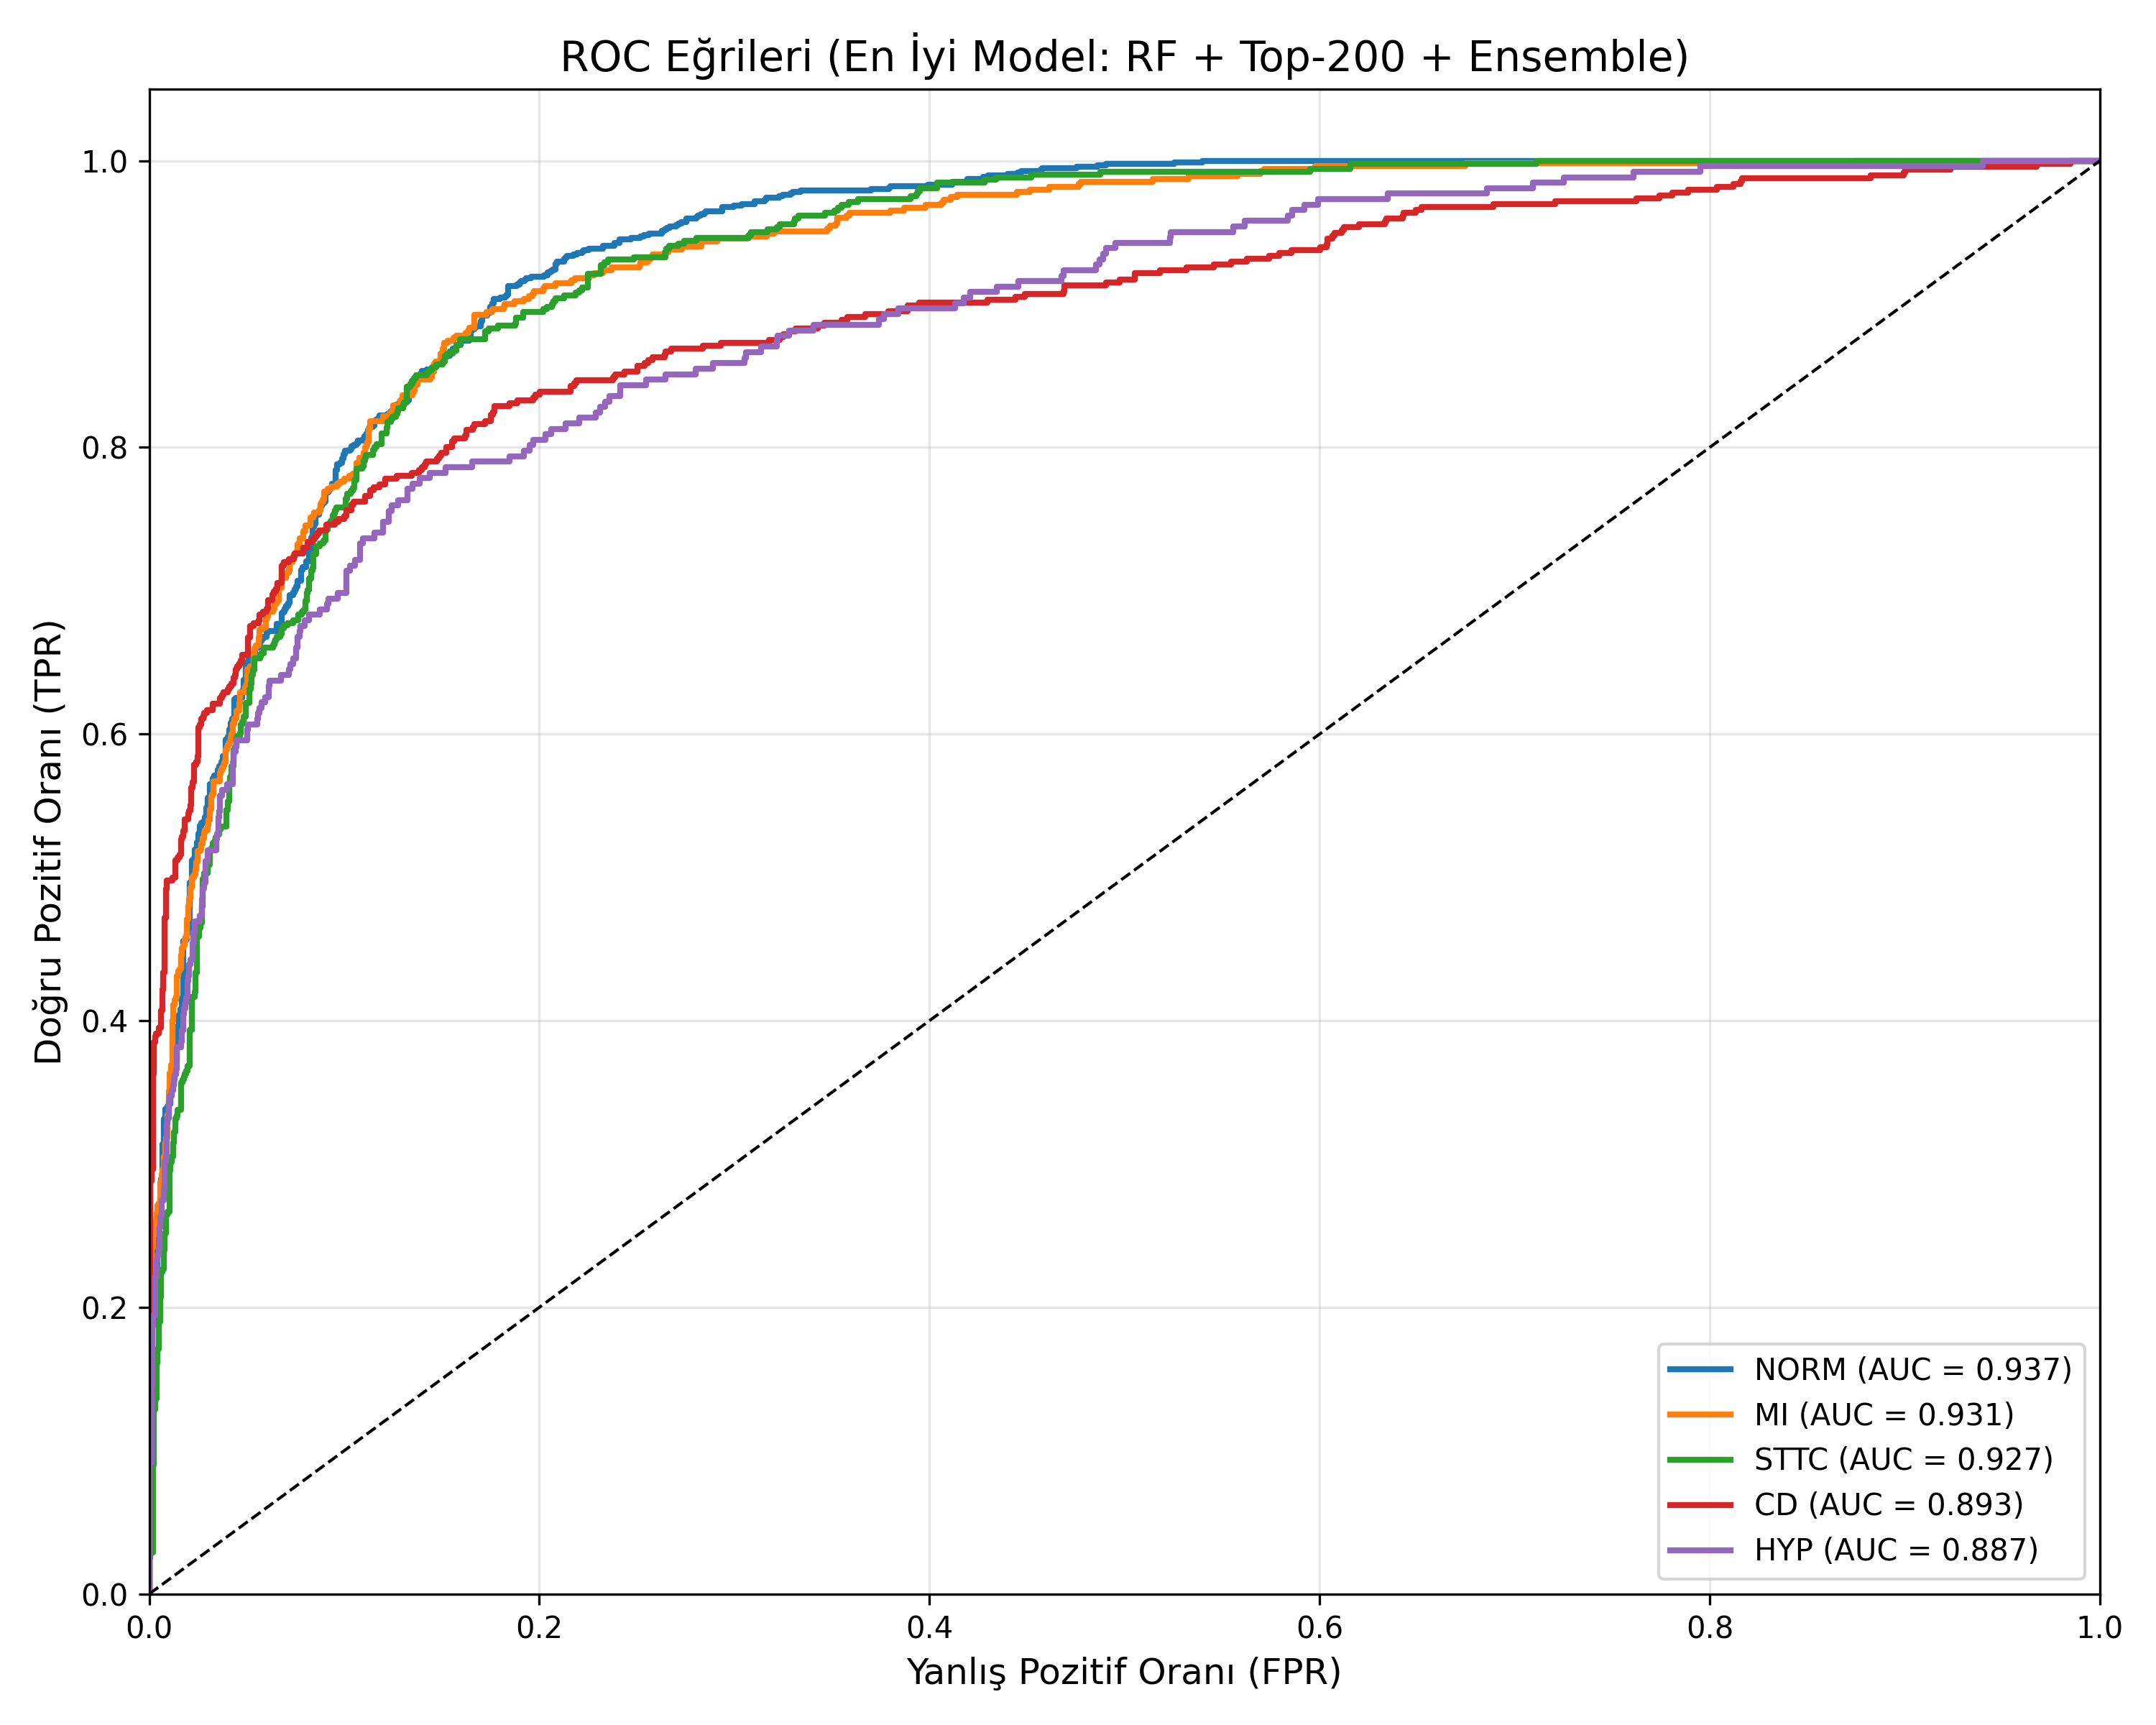
\includegraphics{../reports/model_comparison/roc_curves_final.png}}
\end{frame}

%=================================
\section{Tartışma ve Gelecek Çalışmalar}

\begin{frame}{Tartışma}
	\begin{itemize}
		\item PTB-XL+ veri seti üzerinde 5 üst sınıf (NORM, MI, STTC, CD, HYP) için RF tabanlı bir sınıflandırma hattı kurulmuştur.
		\item Eksik verilerin rastgele dağılmadığı, özellikle P dalgası ile ilgili özniteliklerde MI ve STTC'de yoğunlaştığı görülmüş; bu nedenle eksiklik, \emph{bilgi taşıyan} bir durum olarak modele dahil edilmiştir.
		\item Öznitelik sayısının artması genel olarak performansı iyileştirmiş; ROC-AUC değerleri 0.90+ bandında seyretmiştir.
		\item Undersampling, recall değerlerini artırsa da precision ve accuracy'de azalmaya yol açmış; sınıf ağırlıkları daha dengeli bir davranış sunmuştur.
	\end{itemize}
\end{frame}

\begin{frame}{Sınıf Bazlı Değerlendirme ve Sınırlılıklar}
	\begin{itemize}
		\item NORM sınıfında yüksek recall elde edilirken, MI ve STTC sınıflarında dengeli F1 değerleri gözlenmiştir.
		\item HYP en zor sınıf olup, hem sınıf örnek sayısının azlığı hem de diğer anomali örüntüleriyle örtüşmesi nedeniyle daha düşük metrikler üretmektedir.
		\item Çalışmanın sınırlılıkları:
		\begin{itemize}
			\item Sınıf dengesizliği yalnızca sınıf ağırlıkları ve basit undersampling ile ele alınmıştır.
			\item Olasılık kalibrasyonu ve karar eşiklerinin klinik hedeflere göre optimize edilmesi detaylı incelenmemiştir.
			\item RF önem skorları belirli yanlılıklara açık olabilir; Top-N kümelerin stabilitesi farklı tohumlarla ayrıca analiz edilebilir.
		\end{itemize}
	\end{itemize}
\end{frame}

\begin{frame}{Gelecek Çalışmalar}
	\begin{itemize}
		\item RF yerine veya yanında XGBoost/LightGBM gibi gradient boosting yöntemlerinin denenmesi.
		\item Dengesizliğe duyarlı topluluk yöntemleri: Balanced Random Forest, EasyEnsemble vb.
		\item Sınıf bazlı eşiklerin, olasılık kalibrasyonu (sigmoid/isotonic) ve klinik kısıtlar (ör. minimum HYP recall) ile birlikte optimize edilmesi.
		\item HYP performansını artırmak için alt sınıf (ör. LVH/RVH) düzeyinde daha homojen etiketleme ve ek vektörkardiyografik özniteliklerin değerlendirilmesi.
	\end{itemize}
\end{frame}
\begin{frame}{Gelecek Çalışmalar (Devam)}
		LLM modellerinden yararlanılarak bu sonuçlar bulunmuştur:

	\begin{itemize}
		\item Ham EKG dalga formu üzerinden 1D-CNN/Transformer tabanlı derin öğrenme modelleri ve klasik özniteliklerle hibrit yaklaşımların karşılaştırılması.
		\item Özellikle azınlık sınıflar için özdenetimli (self-supervised) ön eğitim (ör. contrastive learning) ile temsil öğrenimi ve ardından ince ayar (fine-tuning).
		\item Değerlendirmede hasta-bazlı (patient-wise) bölme, harici veri seti ile genelleme testi ve cihaz/merkez farklılıklarına karşı alan uyarlama (domain adaptation).
		\item Gürültü/artefakt dayanıklılığı: veri artırma (noise, baseline wander), kalite kontrol (signal quality index) ve derivasyon (lead) seçiminin etkisinin analizi.
		\item Açıklanabilirlik ve klinik doğrulama: SHAP/permütasyon önemleri ile kararların yorumlanması ve hata analiziyle (confusion + örnek inceleme) model iyileştirme döngüsü.
	\end{itemize}
\end{frame}
%=================================

\begin{frame}[t]{Süreç Fotoğrafları}
	\centering

	% Top row: two meeting photos (same height so they align and fit)
	\begin{columns}[T,onlytextwidth]
		\begin{column}{0.49\textwidth}
			\centering
			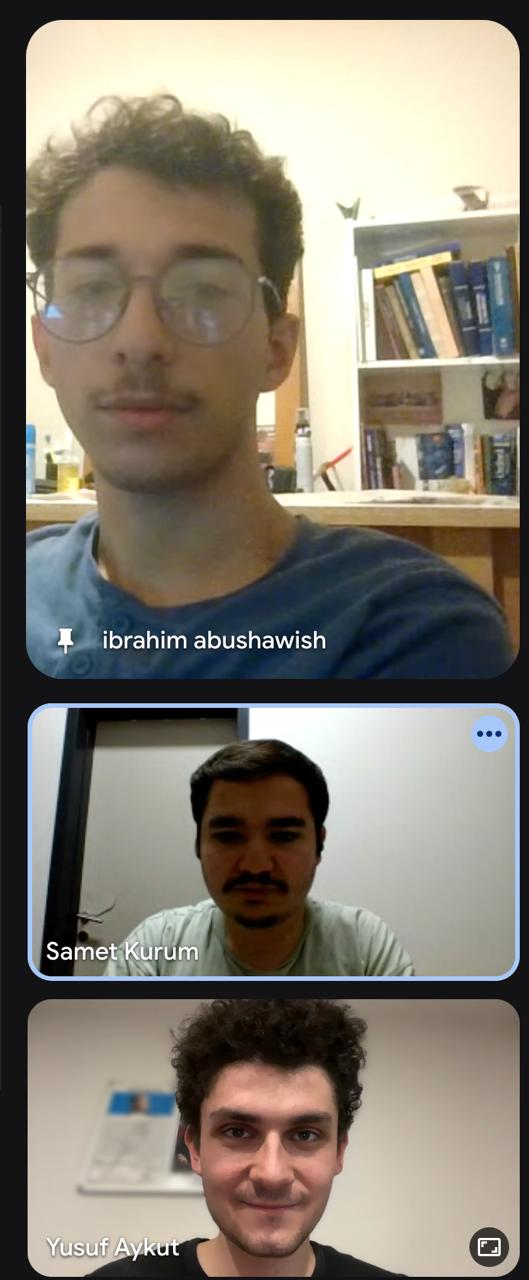
\includegraphics[
				width=\linewidth,
				height=0.7\textheight,
				keepaspectratio
			]{meeting_photo_1.png}\\[-2pt]
			\scriptsize Toplantı 1
		\end{column}

		\begin{column}{0.49\textwidth}
			\centering
			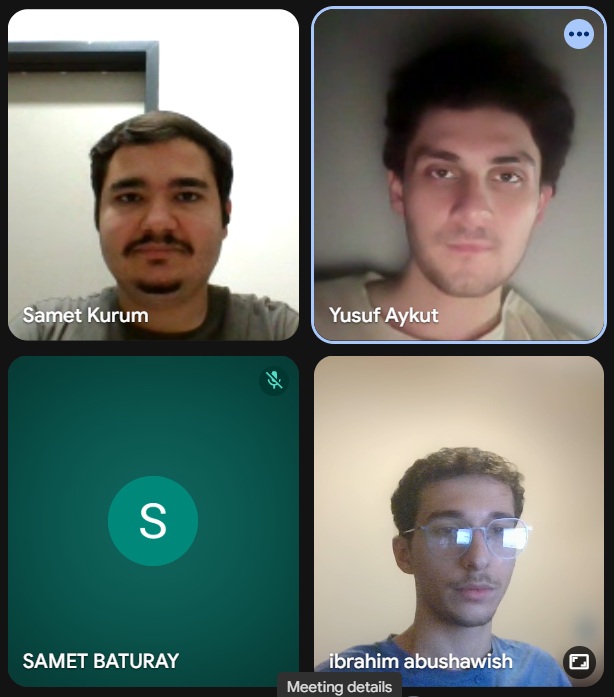
\includegraphics[
				width=\linewidth,
				height=0.7\textheight,
				keepaspectratio
			]{meeting_photo_2.png}\\[-2pt]
			\scriptsize Toplantı 2
		\end{column}
	\end{columns}

	\vspace{0.15cm}

\end{frame}

\begin{frame}{Gantt Şeması}
	% Bottom: Gantt (bounded by height to prevent overflow)
	\centering
	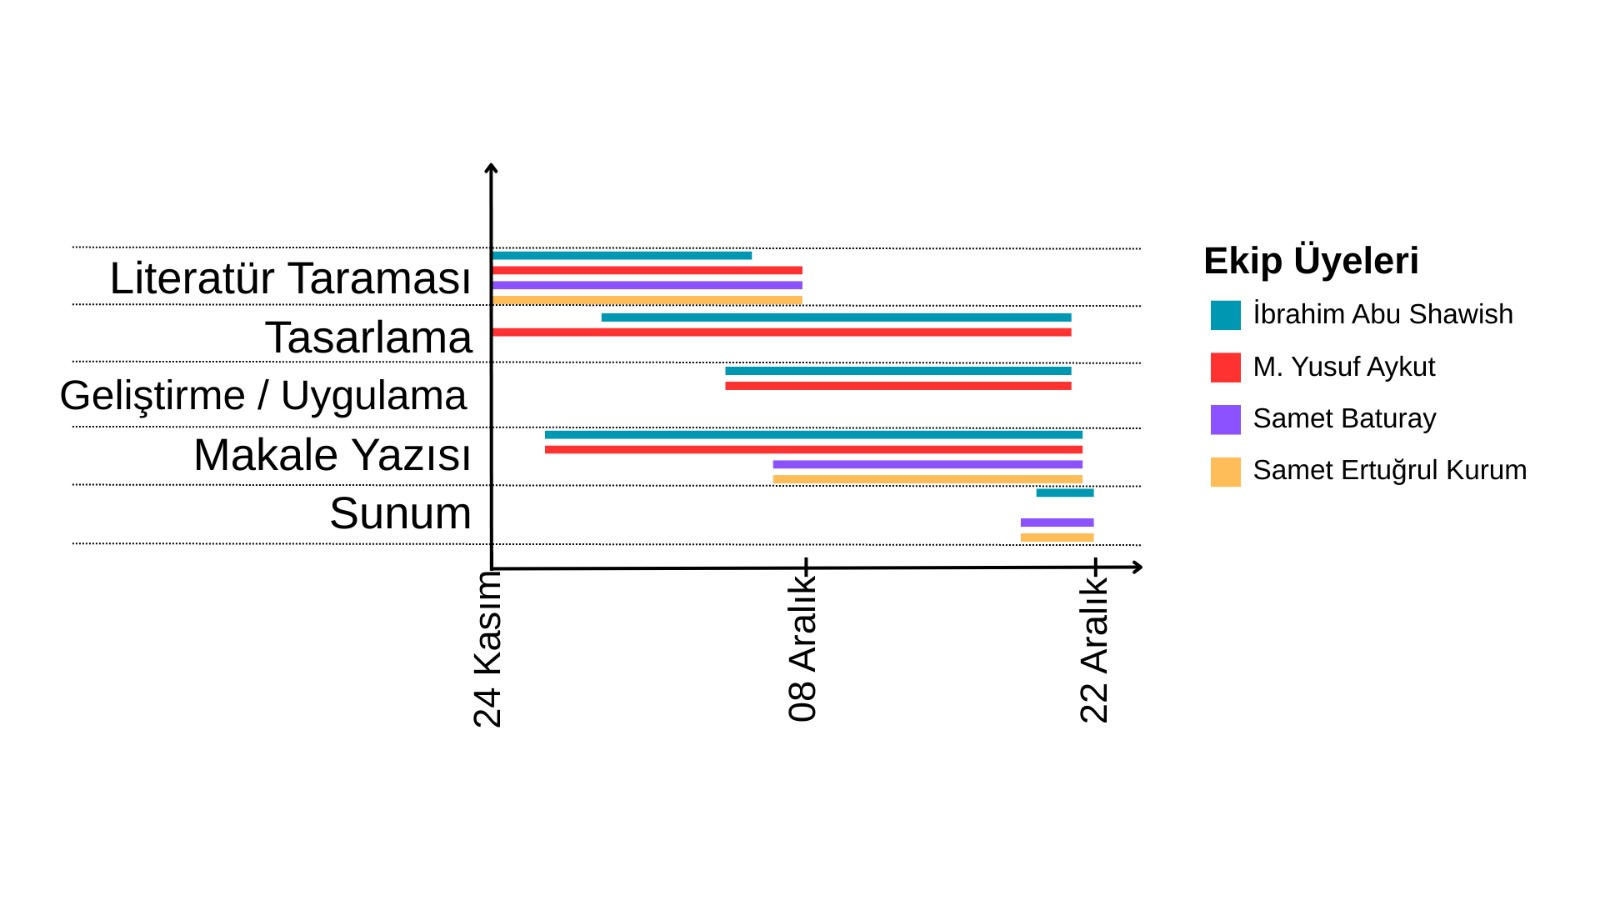
\includegraphics[
		width=\linewidth,
		height=0.8\textheight,
		keepaspectratio
	]{gantt.jpeg}\\[-2pt]
	\scriptsize Proje Gantt Şeması
\end{frame}

\begin{frame}{Beyan}
	\centering
	Bu sunumda yer alan tüm analizler, yorumlar ve sonuçlar \textbf{yazarlar tarafından} gerçekleştirilmiş olup, herhangi bir dış kaynaktan izinsiz alıntı veya intihal içermemektedir.\par\medskip
	Ayrıca, çalışma kapsamında \textbf{kod geliştirme süreçlerinde} ve \textbf{bazı metin bölümlerinin taslaklandırılması/düzenlenmesinde} Büyük Dil Modellerinden (LLM) destek alınmıştır.
	\end{frame}
\section{Referanslar}

\begin{frame}[allowframebreaks]{Referanslar}
	\scriptsize
	\setlength{\parskip}{2pt}
	\setbeamertemplate{bibliography item}{\insertbiblabel}

	\begin{thebibliography}{99}

		\bibitem{taconne2024-lvh}
		M. Taconné, V. D. Corino, \& L. Mainardi,
		\emph{An ECG-Based Model for Left Ventricular Hypertrophy Detection: A Machine Learning Approach},
		IEEE Open Journal of Engineering in Medicine and Biology (2024).

		\bibitem{osterlund2025-mi-ptbxl}
		R. Österlund, \& H. Rekstad,
		\emph{Machine learning models for classification of myocardial infarction using the PTB-XL dataset} (2025).

		\bibitem{raipal2020-xgboost-cinc}
		H. Raipal, M. Sas, C. Lockwood, J. R., N. S. Peters, \& M. Falkenberg,
		\emph{Interpretable XGBoost based classification of 12-lead ECGs applying information theory measures from neuroscience},
		In \emph{2020 Computing in Cardiology} (IEEE, 2020).

		\bibitem{wagner2020-ptbxl}
		P. Wagner, N. Strodthoff, R.-D. Bousseljot, D. Kreiseler, F. I. Lunze, W. Samek, T. Schaeffter,
		\emph{PTB-XL, a large publicly available electrocardiography dataset},
		Scientific Data, 7, 154 (2020).
		\url{https://doi.org/10.1038/s41597-020-0495-6}

		\bibitem{wagner2023-ptbxlplus}
		P. Wagner, T. Mehari, N. Strodthoff, et al.,
		\emph{PTB-XL+, a comprehensive electrocardiographic feature dataset},
		Scientific Data (2023).
		\url{https://doi.org/10.1038/s41597-023-02153-8}

		\bibitem{strodthoff2020-benchmarks}
		N. Strodthoff, P. Wagner, T. Schaeffter, W. Samek,
		\emph{Deep learning for ECG analysis: Benchmarks and insights from PTB-XL},
		arXiv preprint arXiv:2004.13701 (2020).
		\url{https://arxiv.org/abs/2004.13701}

		\bibitem{breiman2001-rf}
		L. Breiman,
		\emph{Random forests},
		Machine Learning, 45(1), 5--32 (2001).
		\url{https://doi.org/10.1023/A:1010933404324}

		\bibitem{guyon2003-feature-selection}
		I. Guyon, A. Elisseeff,
		\emph{An introduction to variable and feature selection},
		Journal of Machine Learning Research, 3, 1157--1182 (2003).

		\bibitem{jolliffe2016-pca-review}
		I. T. Jolliffe, J. Cadima,
		\emph{Principal component analysis: A review and recent developments},
		Philosophical Transactions of the Royal Society A, 374(2065), 20150202 (2016).

		\bibitem{strobl2007-rf-importance-bias}
		C. Strobl, A.-L. Boulesteix, A. Zeileis, T. Hothorn,
		\emph{Bias in random forest variable importance measures: Illustrations, sources and a solution},
		BMC Bioinformatics, 8, 25 (2007).
		\url{https://doi.org/10.1186/1471-2105-8-25}

		\bibitem{rubin1976-missing-data}
		D. B. Rubin,
		\emph{Inference and missing data},
		Biometrika, 63(3), 581--592 (1976).
		\url{https://doi.org/10.1093/biomet/63.3.581}

		\bibitem{kuhn2013-applied-predictive-modeling}
		M. Kuhn, \& K. Johnson,
		\emph{Applied Predictive Modeling},
		Springer (2013).

		\bibitem{he2009-imbalanced-data}
		H. He, \& E. A. Garcia,
		\emph{Learning from imbalanced data},
		IEEE Transactions on Knowledge and Data Engineering, 21(9), 1263--1284 (2009).

		\bibitem{liu2008-exploratory-undersampling}
		X.-Y. Liu, J. Wu, \& Z.-H. Zhou,
		\emph{Exploratory undersampling for class-imbalance learning},
		IEEE Transactions on Systems, Man, and Cybernetics, Part B, 39(2), 539--550 (2008).

		\bibitem{sterne2009-multiple-imputation}
		J. A. C. Sterne, I. R. White, J. B. Carlin, M. Spratt, P. Royston, M. G. Kenward, J. R. Carpenter,
		\emph{Multiple imputation for missing data in epidemiological and clinical research: Potential and pitfalls},
		BMJ, 338, b2393 (2009).
		\url{https://doi.org/10.1136/bmj.b2393}
		\bibitem{ibm-random-forest}
		IBM,
		\emph{Random forest},
		IBM Think (erişim: 22 Aralık 2025).
		\url{https://www.ibm.com/think/topics/random-forest}
		\bibitem{cfi-bagging}
		Corporate Finance Institute (CFI),
		\emph{Bagging (Bootstrap Aggregation)},
		(erişim: 22 Aralık 2025).
		\url{https://corporatefinanceinstitute.com/resources/data-science/bagging-bootstrap-aggregation/}
	\end{thebibliography}
\end{frame}

\begin{frame}{Teşekkürler}
	\centering
	\Huge{Sorularınız için teşekkür ederiz.}

	\vfill
	\footnotesize
	\textbf{M. Yusuf Aykut \quad İbrahim Abushawish \quad Samet Ertuğrul Kurum \quad Samet Baturay}
\end{frame}

\end{document}

